\documentclass[]{interact}

\usepackage{epstopdf}% To incorporate .eps illustrations using PDFLaTeX
\usepackage[caption=false]{subfig}% Support for small, `sub' figures and tables
\usepackage[T1]{fontenc}
\usepackage{lmodern}

% Math & graphics
\usepackage{amsmath}
\usepackage{graphicx}

% Additional packages
\usepackage{algorithm}
\usepackage{algpseudocode}
\usepackage{tikz}
\usepackage{booktabs}
\usepackage{threeparttable}
\usepackage{tabularx}
\usepackage{array}
\usepackage{multirow}
\usepackage{float}
\usepackage{placeins}
\usepackage{xcolor}
\usepackage{arydshln}
\usepackage{url}
\usepackage{capt-of}

\usepackage[numbers,sort&compress]{natbib}
\bibpunct[, ]{[}{]}{,}{n}{,}{,}
\renewcommand\bibfont{\fontsize{10}{12}\selectfont}

% Author comment commands (set to black for submission)
\newcommand{\galit}[1]{\textcolor{black}{#1}}
\newcommand{\matt}[1]{\textcolor{black}{#1}}

% Theorem-like environments
\theoremstyle{plain}
\newtheorem{theorem}{Theorem}[section]
\newtheorem{lemma}[theorem]{Lemma}
\newtheorem{corollary}[theorem]{Corollary}
\newtheorem{proposition}[theorem]{Proposition}

\theoremstyle{definition}
\newtheorem{definition}[theorem]{Definition}
\newtheorem{example}[theorem]{Example}
\newtheorem{principle}{Principle}

\theoremstyle{remark}
\newtheorem{remark}{Remark}
\newtheorem{notation}{Notation}

\newenvironment{scenario}[1]{%
  \par\vspace{1ex}\noindent\textbf{#1}\par\vspace{0.5ex}}{\par}

%%%%%%%%%%%%%%%%%%%%%%%%%%%%%%%%%%%%%%%%%%%%%%%%%%%%%%%%%%%%%%%%%%%%%%%%%%%%%%

\begin{document}

\articletype{RESEARCH ARTICLE}

\title{When Will Your Model Fail? TreeAlert: \\ A Method for Predicting Extreme Forecasting Failures}

\author{
%\name{Matthew Bobea\textsuperscript{a}, Galit Shmueli\textsuperscript{a}\thanks{CONTACT Galit Shmueli. Email: shmueli@mx.nthu.edu.tw} and Soumya Ray\textsuperscript{a}}
%\affil{\textsuperscript{a}Institute of Service Science, National Tsing Hua University, Hsinchu, Taiwan}
}

\maketitle

\begin{abstract}
The heavy reliance on time-series forecasting in critical decisions gives rise to an urgent need to address extreme forecasting failures that significantly impact organizations. Such errors can arise due to the nature of forecasting algorithms and their interaction with data patterns. This study distinguishes itself by foregrounding a critical-yet-previously-overlooked question: \emph{when} are models likely to fail? Guided by principles of pattern-based error prediction, we develop TreeAlert, a novel method designed to identify patterns of extreme forecasting errors and predict timings of future extreme failures. TreeAlert uses regression trees to detect failure-prone conditions, linking them to contextual and timing patterns. By forecasting timings of future failures, TreeAlert transforms retrospective error analysis into a forward-looking tool that empowers decision-makers to proactively anticipate vulnerabilities, and for data scientists to improve algorithmic weaknesses. We demonstrate TreeAlert using electricity demand and heart rate data, applying it to point forecasts and forecast distributions. This paper makes several contributions: it introduces a generalizable framework for predicting pattern-based model failures; it presents TreeAlert---a model-agnostic, interpretable, and operationally-integrable method; it proposes the lift metric for model tuning and evaluation; and expands the field of error analysis by shifting focus from error magnitude to predicting timings of likely extreme failures.
\end{abstract}

\begin{keywords}
Error Analysis; Time Series Forecasting; Regression Tree; Machine Learning; Lift; Decision Making
\end{keywords}

%%%%%%%%%%%%%%%%%%%%%%%%%%%%%%%%%%%%%%%%%%%%%%%%%%%%%%%%%%%%%%%%%%%%%%%%%%%%%%
%  MAIN BODY
%%%%%%%%%%%%%%%%%%%%%%%%%%%%%%%%%%%%%%%%%%%%%%%%%%%%%%%%%%%%%%%%%%%%%%%%%%%%%%

\section{Introduction}
\label{sec:Intro}
Modern decisions related to purchasing, marketing, manufacturing, staffing, financial planning, logistics, and emergency medical services often depend on time-series forecasts \citep{abreu2023}. Digital transformation across industries has enabled increasingly diverse and voluminous data collection that, coupled with enhanced granularity, has led to improved forecast accuracy \citep{chae2024}. In parallel, researchers have developed various time series forecasting models and forecasting support systems (FSS)---decision support systems specialized for forecasting---to facilitate forecasting and support decision making \citep{petropoulos2022}.

Yet, the efficacy of decisions derived from these FSSs is bounded by the forecasting model's inherent limitations and our comprehension of those constraints. In spite of their sophistication, even properly tuned forecasting models often produce systematic errors \citep{eyuboglu2022}. These errors reflect deviations of the forecasts from the actual values. If these systematic errors exceed the acceptable threshold for a domain, we call them \emph{patterns of extreme forecast failures}, or simply \emph{extreme failure patterns}.

Predicting potential model failures is crucial for ensuring safety in model deployment, especially for applications with serious consequences \citep{tsiligkaridis2021}. We use the term \emph{failure} to imply errors with practical consequences. Extreme failures can significantly impact organizations by resulting in inaccurate stocking decisions \citep{boylan2021}, pose challenges to the operation and planning of the electricity market \citep{zhu2025}, increased supply chain uncertainty, and result in wasted resources and business failures \citep{chae2024}. Understanding and mitigating these extreme failures is therefore essential, as the consequences affect organizational viability and public safety.

Periods with high-risk of extreme forecast failure present a particular challenge for decision-makers because the reliability of forecasts may degrade under certain conditions, directly undermining the quality of forecast-driven decisions. For example, in emergency medical services operations, demand behavior is influenced not only by the month, day of the week, or hour of  day, but also by contextual information such as weather, population age, and the effect of special days \citep{abreu2023}. When these high risk periods are overlooked, forecasts can fail during critical periods.

Identifying extreme failures conditions allows managers to mitigate risks associated with potential failures, set realistic expectations for a forecasting model's performance, and better communicate the model's reliability and applicability to stakeholders \citep{cakmak2024}. Identifying temporal and contextual predictors could help managers understand when (and possibly why) extreme failures take place, and help them make proactive adjustments during periods of elevated risk. For data scientists, identifying extreme failure patterns can highlight areas where the model requires further refinement, such as incorporating additional training data, feature engineering, or model adjustments \citep{cakmak2024}.

It is challenging to identify risky periods in which extreme forecast failures are likely, because these patterns can be obscured by noise, anomalies, high-dimensional feature spaces, irregular seasonal structures, or the scale and complexity of big data environments. This complexity makes them difficult to detect without data-driven methods. Patterns of extreme forecast failures may arise due to structural complexities in the data or the model's failure to capture regime shifts. For instance, complex seasonal patterns and excessive zero values can contribute to extreme errors. Additionally, models that adjust slowly following very high or low values may produce patterns of extreme errors. Patterns of extreme errors can occur even when standard forecasting models, such as smoothing algorithms, ARIMA and regression models, or more complex neural networks, are properly employed. Current time series forecasting approaches can struggle to detect extreme failures due to data complexity, visualization limitations, and inadequate metrics. Fine-grained data can amplify noise, while aggregation might smooth over systematic errors, obscuring failure patterns. Automated forecasting tools often focus on minimizing some overall error metric, overlooking extreme failure patterns. Traditional error metrics like RMSE favor models that minimize overall error even if they fail consistently during a small number of periods.

Despite the ramifications of extreme failures, predicting and understanding the timing of forecasting failures is currently an underexplored area of research. This work aims to develop a systematic method for addressing these challenges. We begin by examining how temporal and contextual patterns of extreme errors emerge from interactions between model behavior and data structure. Integrating these insights with considerations for managerial decision-making, FSS design, sustainability, and gaps in current forecasting methods, we develop a framework that articulates eight foundational principles for predicting extreme forecast failures. We formalize these principles to not only guide the design of our method but also provide a foundation for the development of future methods that aim to predict the timing and context of model failures.

Guided by this framework, we construct TreeAlert---a methodological artifact that aligns with the eight principles. TreeAlert is designed for predicting the timings and context of extreme failure patterns in time series forecasting. TreeAlert identifies extreme failure patterns with its failure-prone conditions, generates human-readable outputs that enable actionable insights and model improvements, and is capable of predicting the timing and context of future failure periods. TreeAlert utilizes a specially-tailored regression tree, with novel training and evaluation operations. Lastly, TreeAlert adapts the lift metric from the marketing literature to optimize hyperparameter tuning and evaluate how effectively the model prioritizes periods of extreme forecast failure. This assessment ensures the reliability of the method and provides feedback for iterative refinement.

This paper makes several contributions. First, it introduces a generalizable design framework for predicting pattern-based model failures. Second, the novel proposed method focuses on a critical yet previously overlooked question: when are models likely to fail? Building on this shift in perspective, it proposes TreeAlert as a model-agnostic, interpretable, and operationally-integrable method capable of detecting diverse error patterns and predicting periods of extreme model failure. Third, this work makes a theoretical contribution to the machine learning field of error analysis and to the forecasting literature, by reframing error analysis around the question of \emph{when} extreme errors are likely to occur, rather than the traditional focus on error magnitude, thereby opening new avenues for anticipatory decision support in forecasting systems. Finally, this paper addresses the stark absence of fair comparison benchmarks, and positions itself as a foundational reference point for future research on the matter.

\section{Patterns of Extreme Forecast Errors}
\label{sec:patterns}
Prediction errors play a central role in both retrospective and prospective modeling. In retrospective analysis, residuals are examined to assess violated model assumptions, detect outliers, and characterize error distributions. In contrast, our focus is \emph{prospective}.

Literature on \emph{error analysis} examines prediction errors to gain insights into model behavior, weaknesses, and  generalization capabilities \citep{cakmak2024}. Error analysis in machine learning focuses on \emph{categorical} errors, such as false alarms or missed detections, and is most commonly applied to cross-sectional data. By contrast, forecasting errors are \emph{continuous numeric} outcomes, structured in time, and influenced by temporal and contextual dependencies. Moreover, traditional error analysis is largely \emph{retrospective}---identifying the sources and drivers of model error after the fact \citep{cakmak2024}. \matt{It focuses on quantifying error magnitude \citep{kim2020}, characterizing uncertainty through prediction intervals \citep{salem2020}, or developing early warning systems for imminent events \citep{shmueli2010}, rather than predicting when future failures will occur. This represents a critical gap we address.}

A second and more consequential gap concerns \emph{timing}. While the forecasting literature extensively studies error magnitude, it offers little guidance on \emph{when} extreme errors are likely to occur. Anticipating the timing of extreme errors is critical in many domains, enabling advance preparation, resource allocation, and risk mitigation. Examples include healthcare staffing, inventory planning, energy system operations, and emergency response. Yet, existing methods rarely address this prospective question.

Our work aims to fill these two critical gaps. We develop a framework and method for expanding error analysis into time series forecasting, for \textit{forecasting} \textit{when future extreme model failures will occur.} Our focus is \textit{prospective} (future predictions), \textit{temporal} (timing and/or context), and isolates \textit{patterns} of extreme errors (as opposed to anomalies). We define a pattern as \textit{a configuration of temporal and/or contextual} \textit{variables that repeatedly predict extreme errors.} These include temporal information (e.g., day of week, hour of day) and context (e.g. special events, promotions, and weather forecasts).

\renewcommand{\arraystretch}{1.3}

\subsection{Forecasting Extreme Failure Patterns Differs from Anomaly Detection and Early Event Detection}
\label{sec-contrasting}
Our focus in this work is on predicting pattern-based extreme forecasting failures.
Two related but distinct areas are \emph{anomaly detection} and \emph{early event detection}. Anomaly detection focuses on identifying observations that deviate from ``normal'' behavior \citep{chandola2009, nassif2021}. Anomalies typically refer to isolated events rather than recurring patterns and are identified retrospectively to trigger responses such as fraud alerts or infrastructure fault detection \citep{patcha2007, akouemo2016}.
Early event detection shares similarities with anomaly detection in that it identifies deviations from expected behavior, but it emphasizes real-time monitoring to detect emerging disruptions, such as cyberattacks or disease outbreaks \citep{wang2021, deljac2015, shmueli2010}. Table~\ref{tab:contrast} summarizes the key distinctions between these approaches and ours. A central characteristic of both anomaly detection and early event detection is their limited focus on the \emph{timing of extreme values}. Isolated anomalies rarely reveal the conditions under which future failures will recur, limiting their value for preemptive intervention.

Our approach differs by being explicitly \emph{prospective} and \emph{pattern-driven}. We define a \emph{pattern} as a configuration of temporal and/or contextual variables that repeatedly predicts extreme forecast errors. Temporal predictors capture time-based structure (e.g., hour of day, day of week), while contextual predictors capture exogenous conditions such as promotions, special events, or weather. For example, a failure pattern may take the form ``Wednesdays at 8:00 PM during promotional events.'' Rather than detecting one-off deviations, our goal is to forecast when a model is likely to fail under recurring conditions, enabling improvements in model design and decision-making. Accordingly, an important principle for methods that predict extreme forecasting errors is to focus on patterns rather than individual anomalous events.

\begin{table}
\centering
\caption{Forecasting patterns of extreme model failures contrasted with anomaly detection and early event detection: contrasting goal, temporal focus, and pattern of interest}
\label{tab:contrast}
\begin{threeparttable}
\resizebox{\textwidth}{!}{%
\renewcommand{\arraystretch}{1}%
\setlength{\extrarowheight}{4pt}%
\setlength{\aboverulesep}{0pt}%
\setlength{\belowrulesep}{0pt}%
\footnotesize
\begin{tabular}{>{\centering\arraybackslash}p{1.7cm}%
                >{\centering\arraybackslash}p{4.2cm}%
                >{\centering\arraybackslash}p{3.8cm}%
                >{\centering\arraybackslash}p{3.6cm}}
\toprule
& \textbf{Anomaly / Outlier Detection} & \textbf{Early Detection of Events / Early Warning Systems} & \textbf{Forecasting Patterns of Extreme Model Failures} \\
\midrule
\textbf{Goal} &
\textit{Classify} a single (or pattern) of values that deviate significantly from the norm &
\textit{Detect} an environmental change through collection and monitoring of a series &
\textit{Predict the timing and context of extreme forecast errors} based on preexisting \textit{patterns} \\
\hline
\textbf{Temporal Focus} &
\textit{Retrospective}: Identify deviations or anomalies after they occur &
\textit{Real-Time}: Identify emerging patterns that signal the event &
\textit{Prospective}: Predict future failure conditions \\
\hline
\textbf{Pattern of Interest} &
\textit{Individual or a pattern of events} including rare spikes or anomalies caused by unforeseen events &
\textit{Change in the entire series} due to environmental disruption &
\textit{Patterns} of recurring conditions leading to extreme forecast errors \\
\hline
\textbf{Scope of Analysis} &
\textit{Series'} anomalies are classified based on deviations &
\textit{Series'} environment is monitored for changes &
\textit{Forecast errors} are analyzed to uncover patterns \\
\bottomrule
\end{tabular}}
\end{threeparttable}
\end{table}

We can showcase the implications of shifting from an event-driven to a pattern-driven approach by considering a hospital admissions context.  In anomaly detection, we might be
interested in identifying past days with unusually high patient arrivals. In early event detection, we might analyze emerging patterns of unusually high patient arrivals to detect an emerging epidemic. In contrast, we focus on predicting when the forecasting model itself will fail under recurring conditions. Anticipating such periods allows managers to adjust expectations and mitigate the costs of systematic under- or over-forecasting. This shift highlights the need for actionable failure conditions.

\subsection{Why Patterns of Extreme Forecast Failures Arise}

\matt{Designing a method to predict extreme model failures requires first identifying the conditions under which they arise. This ensures that the method targets generalizable structural patterns rather than isolated anomalies. We define an extreme forecasting failure as a large forecast error magnitude without imposing a fixed threshold.  Such failures frequently coincide with peaks or dips in a series \citep{marvin2022}, but also emerge under routine conditions such as sparse data or slow model adaptation. Each distinct drivers carry different operational implications and costs. We therefore identify and examine five scenarios that commonly exhibit patterns of extreme forecasting failures.}

\begin{scenario}{Scenario A: Series with steep peaks and/or dips}
In practice, many time series have extreme seasonal peaks or dips, such as in urban rail passenger flow, electricity demand, and ozone concentration levels  \citep{li2024, amaraouali2023, marvin2022}. Forecasting models often struggle during the series' peaks or dips leading to extreme errors. This is due to bias that prevents capturing the underlying patterns \citep{lin2023}, or smoothing that captures seasonal shape but not magnitude. Figure~1(A) depicts hourly bike usage along with forecasts and forecast errors, taken from a winning model in a city bike-sharing forecasting competition \citep{mohit2020}. This model was selected for its superior performance metrics, yet we see it consistently struggles to capture the pattern of steep peaks, resulting in extreme positive errors.
\end{scenario}

\begin{scenario}{Scenario B: Complex seasonal patterns}
Time series often exhibit complex seasonal patterns \citep{zhao2024}, such as multiple seasonal cycles, high-frequency seasonality, non-integer seasonality, and dual-calendar effects. For instance, \cite{delivera2011} describe a series with two annual seasonal patterns: one based on the Gregorian calendar (365.25 days per year) and the other on the Hijri (Islamic) calendar (354.37 days per year). The Hijri calendar is based on lunar cycles and is on average 10.88 days shorter than the Gregorian calendar. Such dual-seasonal behavior complicates modeling recurring events, such as holidays, when steep peaks or dips in one calendar do not align with those in another unsynchronized calendar. This can result in extreme errors during non-peak or non-dip periods. Figure~1(B) shows how a misaligned holiday at times $t_1$ and $t_2$ can lead to recurring extreme errors during these periods.
\end{scenario}

\begin{scenario}{Scenario C: Capturing spurious signals}
\matt{Noise or outliers in the training data can lead a model overfit an irrelevant pattern in the training data (as shown in Figure~1(C)) and hinder the model's ability to learn meaningful patterns \citep{cakmak2024}. For example, early models used to forecast flu cases using Google Flu Trends overfit to irrelevant search terms like ``high school basketball,'' which coincided with flu season but were unrelated to flu cases. This led to erroneous over-forecasts of flu cases \citep{lazer2014}. Models that fit these spurious signals generate extreme errors by predicting nonexistent peaks or dips during otherwise stable periods.}
\end{scenario}

\begin{scenario}{Scenario D: Sparse data}
Series with many missing or zero values can generate patterns of extreme forecast errors even in the absence of regular peaks or dips. This is common in rare-event series such as earthquakes or intermittent product demand. Prolonged zero-value periods can lead to over-forecasting during stable periods, while models biased toward zero demand can under-forecast when positive demand resumes \citep{wang2024b}. \matt{This would result in extreme errors during peak or dip periods. Intermittent demand often has regular patterns such as in stock keeping units forecasting \citep{nikolopoulos2021}, as well as irregular patterns such as demand for vehicle spare parts \citep{jiang2021}. These dynamics can produce recurring extreme error patterns, as illustrated in Figure 1(D).}
\end{scenario}

\begin{figure}[h!]
\centering
\setlength{\tabcolsep}{2pt}
\renewcommand{\arraystretch}{0.65}
\begin{tabular}{ll}
\hline
\noalign{\vspace{2pt}}
\multicolumn{2}{c}{%

\includegraphics[width=0.45\linewidth, trim={0pt 4pt 0pt 3pt}, clip]{Figures/label.png}} \\
\noalign{\vspace{2pt}}
\hline
\noalign{\vspace{2pt}}
\multicolumn{2}{c}{%
\begin{tabular}[c]{@{\hspace{2pt}}c@{\hspace{2pt}}}
(A) Steep Peaks and Dips\\[-2pt]
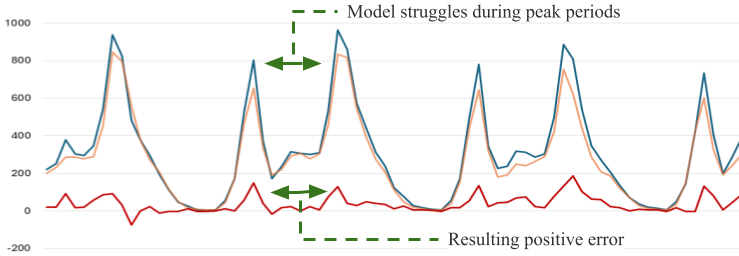
\includegraphics[width=0.75\linewidth]{Figures/1a.png}
\end{tabular}} \\
\noalign{\vspace{2pt}}
\hline
\noalign{\vspace{2pt}}
\begin{tabular}[c]{@{\hspace{2pt}}c@{\hspace{2pt}}}
(B) Complex Seasonal Pattern\\[-2pt]
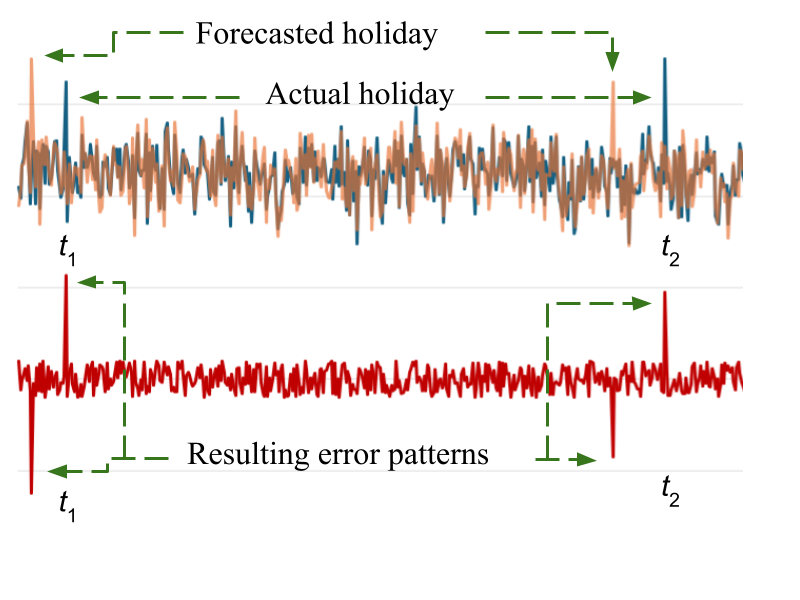
\includegraphics[width=0.40\linewidth, trim={10pt 80pt 80pt 0pt}, clip]{Figures/1b.png}
\end{tabular}
&
\begin{tabular}[c]{@{\hspace{2pt}}c@{\hspace{2pt}}}
(C) Overfit to Spurious Signals or Outliers\\[-2pt]
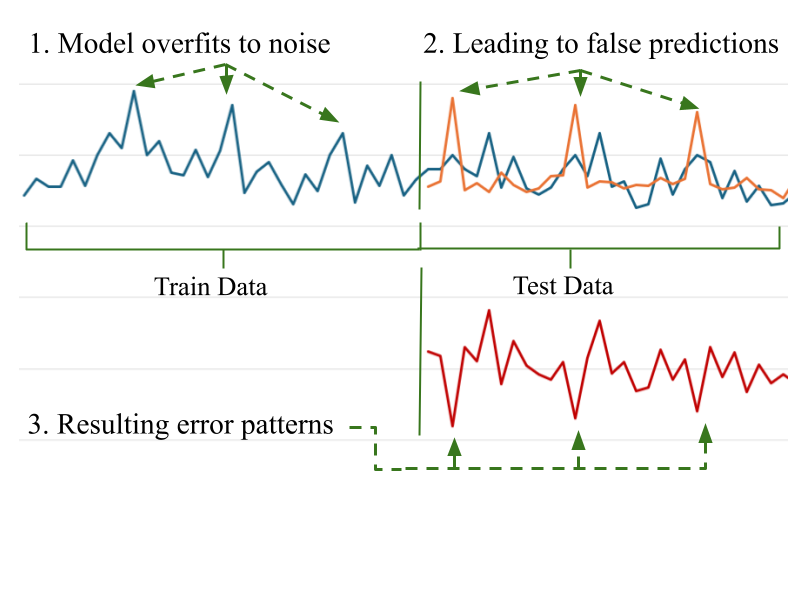
\includegraphics[width=0.45\linewidth, trim={20pt 80pt 20pt 20pt}, clip]{Figures/1c.png}
\end{tabular} \\
\noalign{\vspace{2pt}}
\hline
\noalign{\vspace{2pt}}
\begin{tabular}[c]{@{\hspace{2pt}}c@{\hspace{2pt}}}
(D) Sparse Data\\[-2pt]
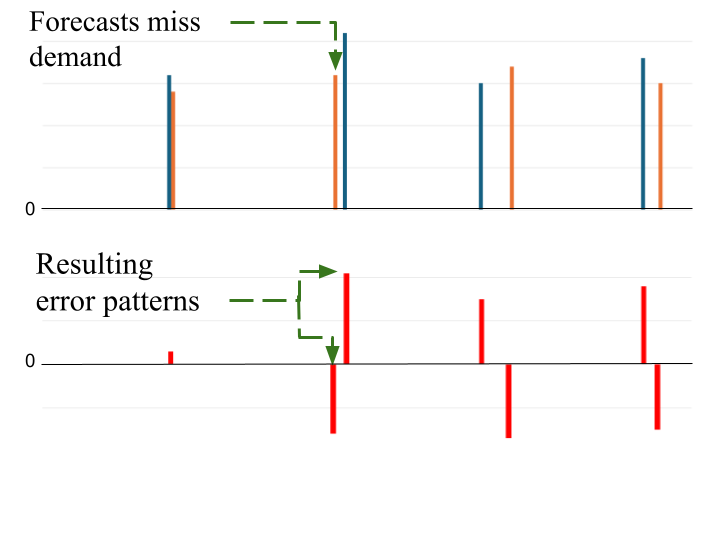
\includegraphics[width=0.43\linewidth, trim={10pt 100pt 20pt 0pt}, clip]{Figures/1d.png}
\end{tabular}
&
\begin{tabular}[c]{@{\hspace{2pt}}c@{\hspace{2pt}}}
(E) Slow-to-Adjust Models\\[-2pt]
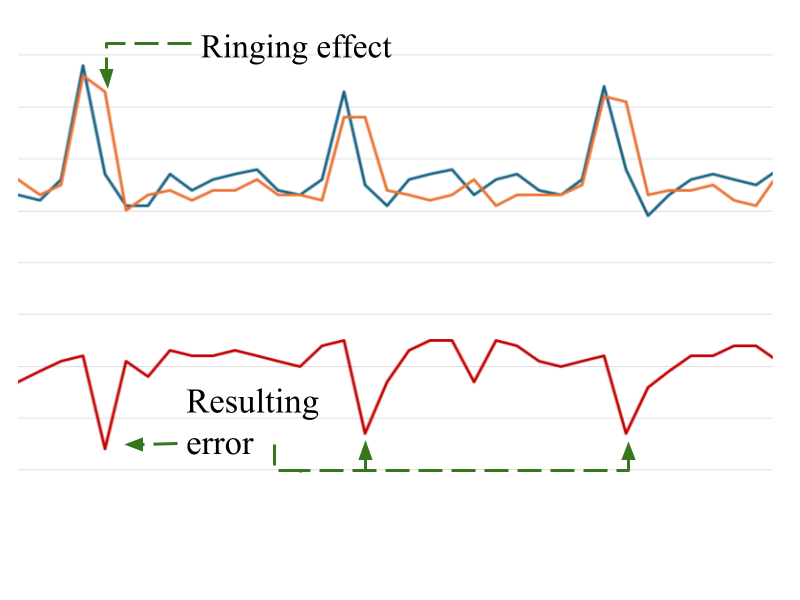
\includegraphics[width=0.43\linewidth, trim={10pt 100pt 20pt 0pt}, clip]{Figures/1e.png}
\end{tabular} \\
\noalign{\vspace{2pt}}
\hline
\end{tabular}
\caption{Five scenarios of extreme forecasting error failure patterns}
\label{fig:error_scenarios}
\end{figure}

\begin{scenario}{Scenario E: Slow-to-adjust models}
Patterns of extreme errors can occur when models fail to adjust after abnormal
peaks or dips, producing a ``ringing'' effect. Such models continue forecasting elevated or reduced values even after conditions stabilize, resulting in large errors during stable periods. For example, a model that captures holiday sales peaks may keep predicting high demand after the holiday ends. As shown in Figure 1(E), these persistent deviations reflect the model's inability to adjust to actual demand.
\end{scenario}

Given these varied scenarios, effective failure prediction methods must capture a broad range of error patterns arising from complex seasonal patterns, sparse data, slow model adjustment, and more.

\subsection{Implications of Extreme Forecasts Failures}

\subsubsection{Extreme Failure Patterns During Peaks and Dips}

In demand forecasting, models that produce extreme failures during peaks and dips (Scenarios A and B) often have more severe consequences than those from models with similar overall error magnitudes spread evenly over time, even if those models perform worse on conventional accuracy metrics.

For example, in supply chain management, disbursed forecast errors allow firms to operate within existing buffers, minimizing demand signal distortion and reducing the likelihood of overreaction. In contrast, failures during peak demand overwhelm safety stocks and trigger stockouts \citep{bray2019}. Persistent under-forecasting during peaks and over-forecasting during dips erodes managerial trust in forecasting systems. This failure prompts downstream overordering, distorting supply chain signals and amplifying the bullwhip effect \citep{croson2014, wu2006}. Consequently, extreme errors during missed peaks and dips generate two distinct trust deficit: one between buyers and sellers, and another between managers and their forecasting systems.

\subsubsection{Extreme Failure Patterns During Non-Peaks/Dips}

Extreme errors that manifest during low variance periods are especially unexpected, and can significantly affect operations. In healthcare, overfitting to spurious correlations (Scenario C) can create false demand spikes, prompting premature mobilization of staff or medical resources. Sparse or intermittent data (Scenario D) can also induce extreme over-forecasts during low-demand periods. Nikolopoulos et al.~\cite{nikolopoulos2021} identified these risks in other fields: overestimating natural disasters leads to burdensome regulation, while over-forecasting market crashes triggers expensive, redundant hedging. Scenario E illustrates a similar problem through the ``ringing effect,'' where models are slow to adjust after high-demand events. Burkom et al.\cite{Burkom2007} found that forecasting models of emergency room visits continued predicting elevated counts after holidays, leading to overstaffing and unnecessary costs.

\subsection{The Limitation of Conventional Performance Metrics}
\matt{Forecasting modelers use metrics such as MAPE and RMSE to benchmark accuracy or define a loss function \citep{petropoulos2022}. Letting $e_t = y_t - F_t$ denote the period-$t$ error, both metrics aggregate over all $T$ periods:
\begin{equation}
\text{MAPE} = \frac{1}{T} \sum_{t=1}^{T} \left| \frac{e_t}{y_t} \right| \times 100,
\qquad
\text{RMSE} = \sqrt{\frac{1}{T} \sum_{t=1}^{T} e_t^2}.
\end{equation}
Because each $e_t$ has equal weight $\frac{1}{T}$, rare but extreme deviations are diluted by the dominant presence of low-magnitude errors, biasing model selection toward overall accuracy at the expense of high-impact periods.}

Figure~\ref{fig:Monthly Sales} illustrates this with artificial monthly sales data exhibiting December holiday surges. As Table~\ref{tab:metrics} shows, Model~1 dominates on all global metrics yet fails to capture December peaks; Model~2 captures those peaks but scores worse overall. Recent advances in peak electricity demand forecasting have introduced loss functions to improve prediction accuracy during peak demand periods \citep{nygard2025}. While these approaches enhance model sensitivity to peaks, their evaluation remains anchored to global metrics that do not isolate local performance.

\FloatBarrier

\begin{figure}[H]
  \centering
  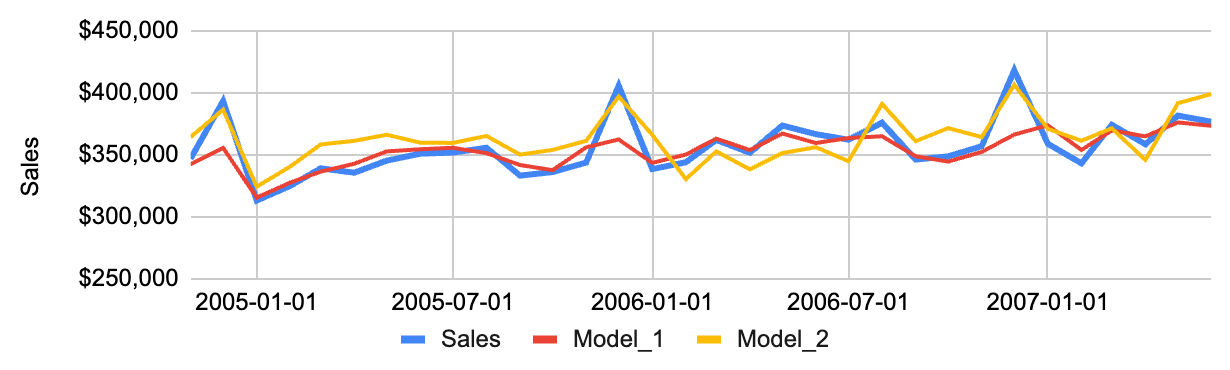
\includegraphics[width=.95\linewidth]{Figures/MonthlySales.png}
  \caption{Monthly sales (hypothetical data) with two forecasting models}
  \label{fig:Monthly Sales}
\end{figure}

\begin{table}[H]
\tbl{Performance metrics for Model 1 and Model 2. All Model 1 metrics are lower (better)}
{\begin{tabular}{lcccccc} \toprule
 & \textbf{ME} & \textbf{RMSE} & \textbf{MAE} & \textbf{MPE} & \textbf{MAPE} & \textbf{MASE} \\
\midrule
\textbf{Model 1} & 2850.04 & 14938.83 & 9069.2  & -0.614 & 2.4174 & 0.4203 \\
\textbf{Model 2} & -6536.35 & 15694.96 & 14586.29 & 1.9647 & 4.1411 & 0.676 \\
\bottomrule
\end{tabular}}
\label{tab:metrics}
\end{table}

\subsection{Design Principles for Pattern-Based Failure Prediction}
\label{subsec-principles}
We have identified key sources that give rise to patterns of extreme forecast failures, the operational implications of lacking advance alerts for their timing, and the limitations of conventional performance metrics in such settings. Building on these insights, and on our temporal--contextual definition of a pattern, we identify eight guiding principles for developing and evaluating methods that predict patterns of future extreme forecast failures. Table \ref{tab:principles} summarizes the eight principles we uncovered in our search to create methods to foresee and interpret extreme forecasting failures. The first five consider the timing of forecasting failures, and the last two emphasize generalizability and operationalization.

The principles of pattern-focus (P1) and diverse error patterns (P3) empower the method to detect systemic failure conditions while accommodating varied sources of error. Actionability (P2) and transparency (P4) address the need for interpretable outputs that allow for timely intervention. Prospective (P5) and local performance (P6) ensure that methods are forward-looking and evaluated on their ability to prioritize extreme failures rather than overall accuracy. Model-agnosticism (P7) and operational integrability (P8) support robustness, adaptability, and scalability, ensuring that forecasting failure methods remain effective across varied algorithms, data characteristics, and system environments.

\begin{table}
\tbl{\textit{Guiding Principles for Methods that Forecast Forecasting Failures.}}
{\begin{tabular}{m{2.3cm}m{11.2cm}} \toprule
\centering\textbf{Principle 1:} \\ \centering\textit{Pattern-focus} & Methods for predicting extreme forecasting failure should focus on patterns \\
\midrule
\centering\textbf{Principle 2:} \\ \centering\textit{Actionability} & Predicted failures should be stated in actionable form to enable proactive intervention before high-risk periods unfold \\
\midrule
\centering\textbf{Principle 3:} \\ \centering\textit{Diverse Error Patterns} & Methods for predicting extreme forecasting failures should accommodate a diverse range of error patterns \\
\midrule
\centering\textbf{Principle 4:} \\ \centering\textit{Transparency} & Methods addressing extreme failures should produce human interpretable explanations of the conditions leading to model failure \\
\midrule
\centering\textbf{Principle 5:} \\ \centering\textit{Prospective} & Methods for predicting forecasting failures should be prospective in nature \\
\midrule
\centering\textbf{Principle 6:} \\ \centering\textit{Local Performance} & Methods for predicting patterns of forecasting failures should optimize local performance during extreme failures, rather than overall performance \\
\midrule
\centering\textbf{Principle 7:} \\ \centering\textit{Model-agnostic} & Methods should function reliably across forecasting methods without being undermined by model-specific properties \\
\midrule
\centering\textbf{Principle 8:} \\ \centering\textit{Operational Integrability} & The method should be easy to integrate into existing systems without imposing significant computational burdens \\
\bottomrule
\end{tabular}}
\label{tab:principles}
\end{table}

These principles provide a coherent foundation for designing failure-prediction methods that are prospective, interpretable, and operationally useful. Collectively, these design-oriented principles address critical gaps in both the error analysis and forecasting literature, and serve as the basis for creating targeted, interpretable, and anticipatory methods to learn from and preempt forecasting failures.

\section{TreeAlert: A Method for Predicting Patterns of\\Extreme Forecasting Failures}
\label{sec:treealert_method}

Based on the eight principles in Section \ref{subsec-principles}, we developed TreeAlert, a novel method designed to identify patterns of extreme forecasting errors and predict the timing and context of future extreme failures. Our proposed approach combines machine learning, statistical techniques, and visualization to support human decision-making by extracting and presenting interpretable rules and visual insights. We name our method TreeAlert, as it relies primarily on extracting rules from a regression tree. Figure \ref{fig:TreeAlertSteps} illustrates the seven methodological steps comprising the TreeAlert method. The input to TreeAlert is a series of forecast errors and their associated timestamps. The forecast errors are the differences between the actual time series values and their forecasts, where forecasts can be generated using any forecasting algorithm. Each step is articulated in the following subsections.

\begin{figure}[t]
  \centering
  \small
  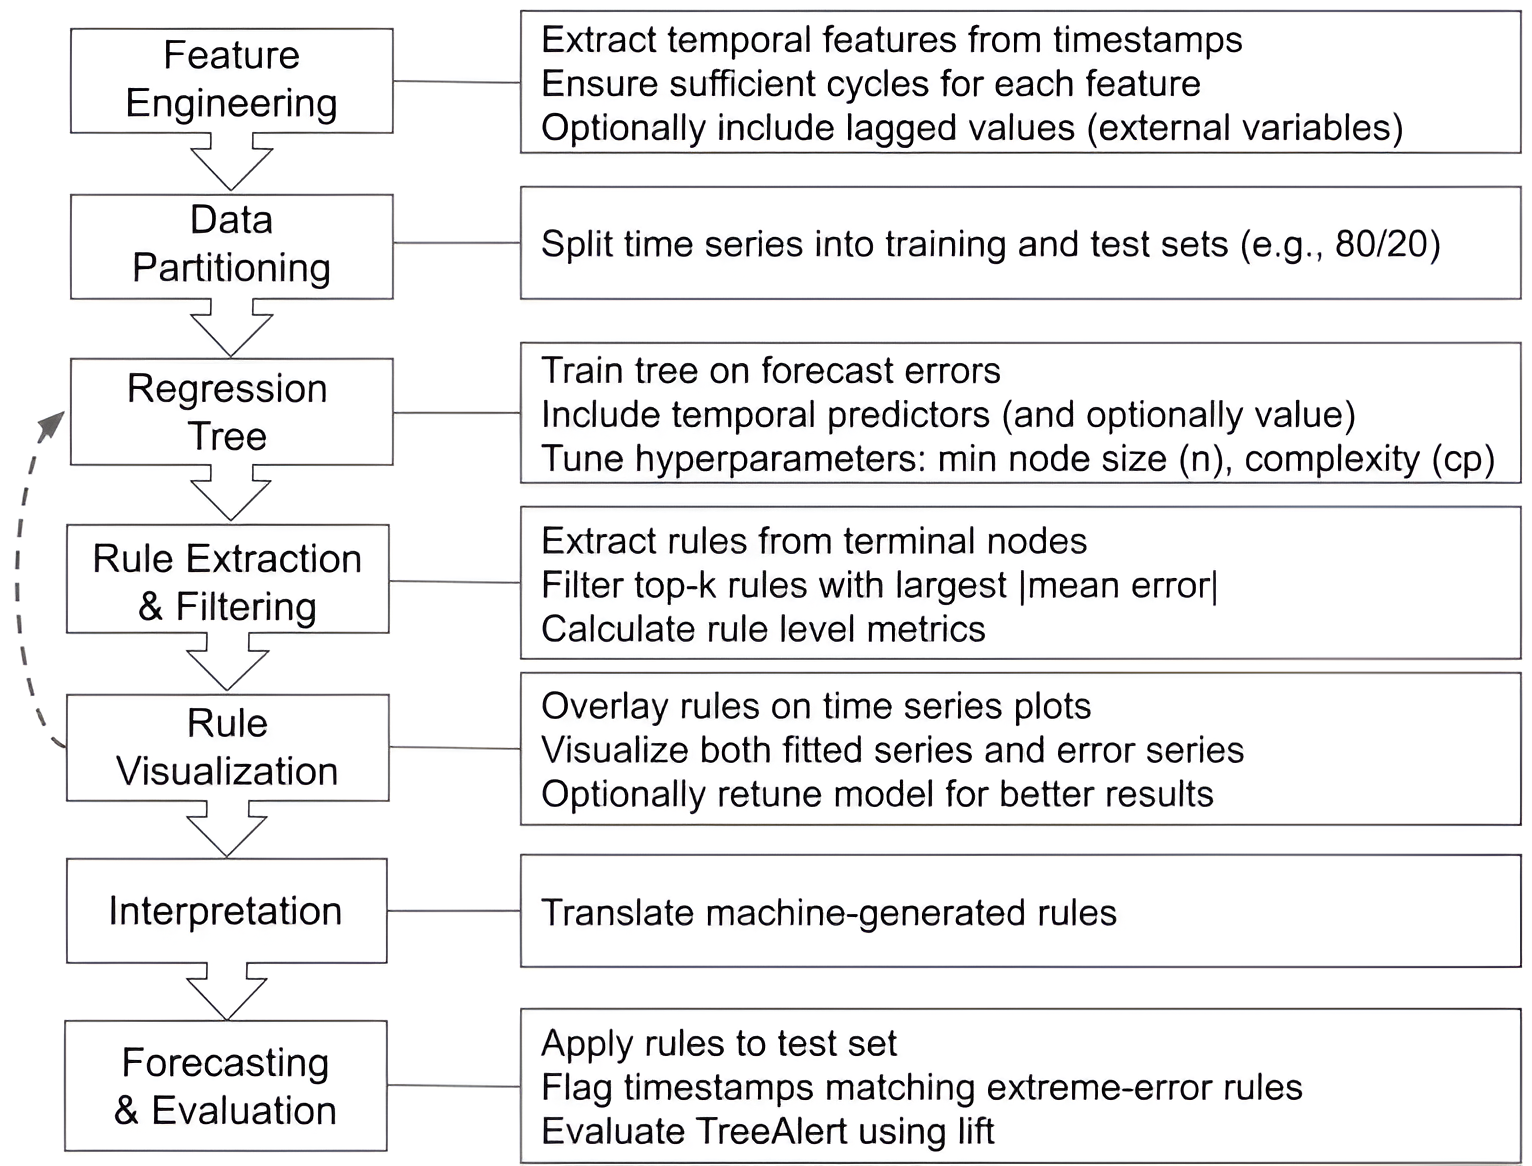
\includegraphics[width=.86\textwidth]{Figures/Tree_alert_chart.png}
  \caption{Diagram of TreeAlert's methodological process}
  \label{fig:TreeAlertSteps}
\end{figure}

\subsection{Step 1 - Feature Engineering}

\matt{TreeAlert is parsimonious, requires only the error series and its associated timestamps, though additional contextual data can also be incorporated. The first step extracts temporal variables (``predictors'') from the timestamps, thereby creating variables such as the month of the year, day of the week, hour of the day, and holiday/non-holiday. This choice is not trivial. The level and number of created predictors is determined by the length and granularity of the test set (see Step 2) so that we have at least two cycles (and ideally more than two) for each relevant predictor.  For instance, ``month of year'' requires at least two years of monthly data; ``hour of day'' requires at least two days of hourly data.}

\subsection{Step 2 - Data Partitioning}

\matt{Before training the tree model, the forecast error series is divided into training ($y_1, \ldots, y_T$) and test subseries ($y_{T+1}, y_{T+2}, \ldots$). The earlier subseries serves as the training set and is
used for training and tuning TreeAlert. The subsequent subseries serves as the test set and is used for evaluating TreeAlert's predictive performance \citep{shmueli2024}.}

Both training and test periods should be sufficiently long to support training and evaluation.
A longer training subseries $y_1, \ldots, y_T$ allows TreeAlert to capture more diverse error conditions.
The length of the test subseries is crucial for properly evaluating TreeAlert's performance---the test set length affects the likelihood that conditions learned during training reappear when testing. For instance, consider a rule learned during training ``extreme over-forecast likely on April 1''. If the test set does not include April 1, then this rule will not trigger an alert. This lack of alerted test periods makes it impossible to assess the rule's generalizability to future periods.

\subsection{Step 3 - Regression Tree}
We apply a regression tree to the training series of forecast errors (the output variable) as a function of temporal and (optionally) contextual predictors. This special output variable highlights our focus on error analysis, in contrast to standard forecasting models that are applied to the original series. The resulting tree structure consists of terminal nodes where forecast errors of similar magnitude and sign are grouped together based on the values of the temporal and contextual predictors.

Once the tree is constructed, TreeAlert departs from conventional regression tree use. Each terminal node represents a distinct combination of temporal and contextual predictors linked to a specific group of forecast errors. The resulting tree may contain numerous terminal nodes. However, unlike standard regression tree applications that display the entire tree for prediction purposes, TreeAlert's branches only lead to terminal nodes that exhibit extreme negative or positive errors (see Section~\ref{sec:rule-extraction} for details). In Step 3, our attention is directed solely toward these terminal nodes and their tree paths.

\subsubsection{Feature Selection}
Choosing too many predictors and/or predictors with high cardinality (e.g., day of month, minute of hour) can lead to overfitting the training period. Such overfitting can lead to rules that focus on overly localized patterns in the training period instead of on patterns that generalize to future periods.

In combination with temporal predictors, TreeAlert can also incorporate contextual predictors. These exogenous features are particularly valuable for identifying and predicting error patterns that arise from interactions between the forecasting model and environmental conditions. For example, the contextual predictor `sales promotion' may capture errors that result from peaks and dips. `Lunar New Year' may capture error patterns from complex lunar seasonal patterns. Contextual predictors must be known (or forecastable) at the time the failure prediction is made to ensure they are valid inputs in prospective applications. A contextual predictor that is highly correlated with temporal variables (e.g., `outdoor temperature' and `time of day') or with another contextual predictor (e.g., `number of walked steps' and `exercise intensity') might be redundant. The regression tree will select the most informative predictor and its values to split on.

\matt{Including the series magnitude as a predictor for capturing errors during peaks and dips is infeasible as future magnitudes are unknown at prediction time. Subject to forecast horizon restraints, lagged values provide a viable alternative as they preserve recent magnitude information, respecting temporal constraints, and capture autoregressive structure.}

\subsubsection{Hyperparameter Tuning and Optimization Using Lift}
\label{sec:tuning_optimization}

\matt{Key hyperparameters include the cost complexity parameter ($cp$), and minimal terminal node size ($n$). Together, they balance under-detection (underfitting) and false detection (overfitting). A small $n$ allows for the identification of nuanced behaviors resulting from temporal and contextual combinations that lead to (possibly few) large errors. A low $cp$ value facilitates more splits in the regression tree, resulting in a more complex model that captures more intricate error patterns. For shorter series or settings with few extreme-error patterns, a smaller $(n, cp)$ improve sensitivity to rare but large errors.}

\matt{Unlike conventional regression tree applications that optimize a global loss function (e.g., $\min \text{MSE}$), TreeAlert tunes hyperparameters by maximizing \emph{lift} for a continuous outcome. Lift is useful for identifying a subset of records that gives the highest cumulative predicted values \citep{shmueli2024machine}. While lift is typically applied to binary outcomes in classification and risk modeling, TreeAlert computes lift on the magnitude of forecast errors, treating error severity as the outcome of interest. This measures how effectively the model concentrates extreme forecast errors for a targeted high-risk segment of periods relative to a random selection of periods. To calculate lift, observations are ranked by predicted error severity $|\hat{e}_t|$ and partitioned into equal-sized quantile subsets (e.g., deciles or ventiles), each containing \( n_g \) observations. }

\matt{To calculate lift, observations are ranked by predicted error severity $|\hat{e}_t|$. They are then partitioned into equal-sized quantile subsets (e.g., deciles or ventiles), each containing \( n_g \) observations. Consistent with TreeAlert's objective of prioritizing the most extreme errors, we focus on lift computed for the highest-ranked subset, denoted \( g_{1} \), which contains the observations with the largest predicted error severity. Let \( n_{g_1} \) denote the number of observations in the highest-ranked subset \( g_{1} \). Once this subset is formed, lift measures the ratio between the average error magnitude within this subset (MAE of $g_1$) and the average  error magnitude across the full period (overall MAE).\footnote{For hyperparameter tuning the full period is the training period; for evaluation, we use the test period.} Lift therefore measures the degree to which this subset concentrates extreme errors relative to the full period. Using \( T \) to denote the total number of observations in the full period, we compute lift for subset \( g_{1} \) as:
\begin{equation}
\text{Lift}(g_{1}) =
\frac{
\displaystyle \frac{1}{n_{g_1}}\sum_{t\in {g_1}} |e_t|
}{
\displaystyle \frac{1}{T}\sum_{t=1}^{T} |e_t|
} = \frac{MAE_{g_1}}{MAE}.
\end{equation}
When error magnitude translates directly into meaningful cost units (e.g., lost revenues or wasted resource units), $\text{Lift}(g_1)$ quantifies the concentration of loss captured by TreeAlert's rules relative to not using rules. Maximizing lift thus prioritizes operationally critical failure periods over overall predictive
accuracy.}

\subsubsection{Extension to Probabilistic Forecasting}

While point forecasts are extremely popular in practice, there has been a move towards probabilistic forecasts in academia. TreeAlert can be used in either scenario. When predictive intervals or distributions are available, extremeness is defined using a probabilistic loss function, and TreeAlert is trained on the resulting scores in place of point-forecast errors. This allows TreeAlert to identify patterns of systematically poor probabilistic performance, such as intervals that are excessively wide or fail to achieve nominal coverage.

In the following we briefly describe what is a probabilistic forecast and how TreeAlert is modified for probabilistic forecasts. An illustration of such a usage applied to the heart-rate series can be found in  Appendix~\ref{probabilistic_treealert}.
\newline
\noindent\textbf{Probabilistic Loss Function}
Let $F_t$ denote the predictive distribution at time $t$, and let $y_t$ denote the observed value.
Define the probabilistic forecast loss at time $t$ as
\begin{equation}
S_t = S(F_t, y_t),
\end{equation}
where $S$ is a probabilistic forecast loss function. Such loss functions are minimized in expectation when the predictive distribution coincides with the true data-generating distribution. A large $S_t$ therefore indicates poor probabilistic forecast performance at time $t$. For example, the Winkler score based on the central $1-\alpha$ interval of $F_t$, with lower bound $L_t$ defined by the $\alpha/2$ quantile and upper bound $U_t$ defined by the $1-\alpha/2$ quantile of $F_t$, is:
\begin{equation}
S_t =
\begin{cases}
U_t - L_t
& \text{if } y_t \in [L_t, U_t], \\[3pt]
(U_t - L_t) + \frac{2}{\alpha}(L_t - y_t)
& \text{if } y_t < L_t, \\[3pt]
(U_t - L_t) + \frac{2}{\alpha}(y_t - U_t)
& \text{if } y_t > U_t.
\end{cases}
\end{equation}
This loss increases when prediction intervals are excessively wide or
when the observed value falls outside the intended coverage region.
\newline
\noindent\textbf{Application of TreeAlert to Probabilistic Forecasting} To apply TreeAlert to probabilistic forecasts, the same seven-step procedure described in Section 3 is followed, replacing the forecast error--based target with the probabilistic forecast loss $S_t$. The regression tree is estimated using $S_t$ in place of the forecast error--based target $|e_t|$. Terminal nodes with large mean values of $S_t$ identify patterns and rules associated with systematically poor probabilistic forecast performance. For new observations, predicted loss severity is assigned based on the corresponding terminal-node mean, and observations are ranked accordingly. Quantile subsets are formed as in the original procedure, and via lift is computed using $S_t$ instead of the forecast error magnitude. Lift for subset $g_{1}$ is defined as:
\begin{equation}
\text{Lift}(g_{1}) =
\frac{
\displaystyle \frac{1}{n_{g_1}} \sum_{t \in g_{1}} S_t
}{
\displaystyle \frac{1}{T} \sum_{t=1}^{T} S_t
}.
\end{equation}
Lift therefore measures the degree to which the highest-ranked subset concentrates elevated probabilistic forecast loss relative to the full evaluation period. Thus, TreeAlert's framework remains structurally unchanged. Only the metric used to capture extremeness is replaced.

\subsection{Step 4 - Rule Extraction and Filtering}
\label{sec:rule-extraction}
Each terminal node in the tree is associated with a tree path that determines its rule. We can present these rules as an unstructured table of rules, one for each node. A rule consists of the combination of temporal (and possibly contextual) predictor values that lead to that terminal node, along with the mean error in that node. An example of a rule might be:
\begin{center}
\textit{``Mean error = 35.85 when Hour is 5 or 16 \& DayofWeek is 1 or 2''}
\end{center}

To isolate extreme errors, we adapted a vertical pruning technique by \cite{danks2024composite} that fundamentally differs from traditional pruning approaches. Rather than removing splits to minimize overall prediction error, this approach selectively retains only the terminal nodes with the highest error magnitudes. The result is a ``hollowed out'' tree structure, where the central portion that contains nodes with smaller errors is removed, while the outer branches that lead to extreme errors are preserved see Figure \ref{fig:tree}. Unlike traditional post-pruning methods that focus on minimizing overall prediction error across all terminal nodes, this method directly filters the terminal nodes based on their individual error magnitudes to focus the model's attention on the outer branches where high-magnitude errors are concentrated. The hollowed-out tree is operationalized in TreeAlert by retaining only the top-$k$ terminal nodes with the largest absolute mean errors, where each retained node contains $n$ or more forecast errors.\footnote{If positive and negative errors carry asymmetric costs, or domain expertise necessitates, one can retain the top $k_1$ negative and top $k_2$ positive mean errors, where $k_1 + k_2 = k$ (see Supplemental Material 4).} This yields $k$ rules that are subsequently used to generate alerts for future periods.

Figure~\ref{fig:tree} illustrates the ``hollowed out'' tree procedure graphically: the shaded region is trimmed to isolate the outer branches corresponding to the most extreme over- and under-forecasting patterns. Retaining only $k$ terminal nodes and their associated rules ensures interpretability by avoiding the complexity of large regression trees that result from high-dimensional features or high-cardinality categorical predictors.

\begin{figure}[ht]
\centering
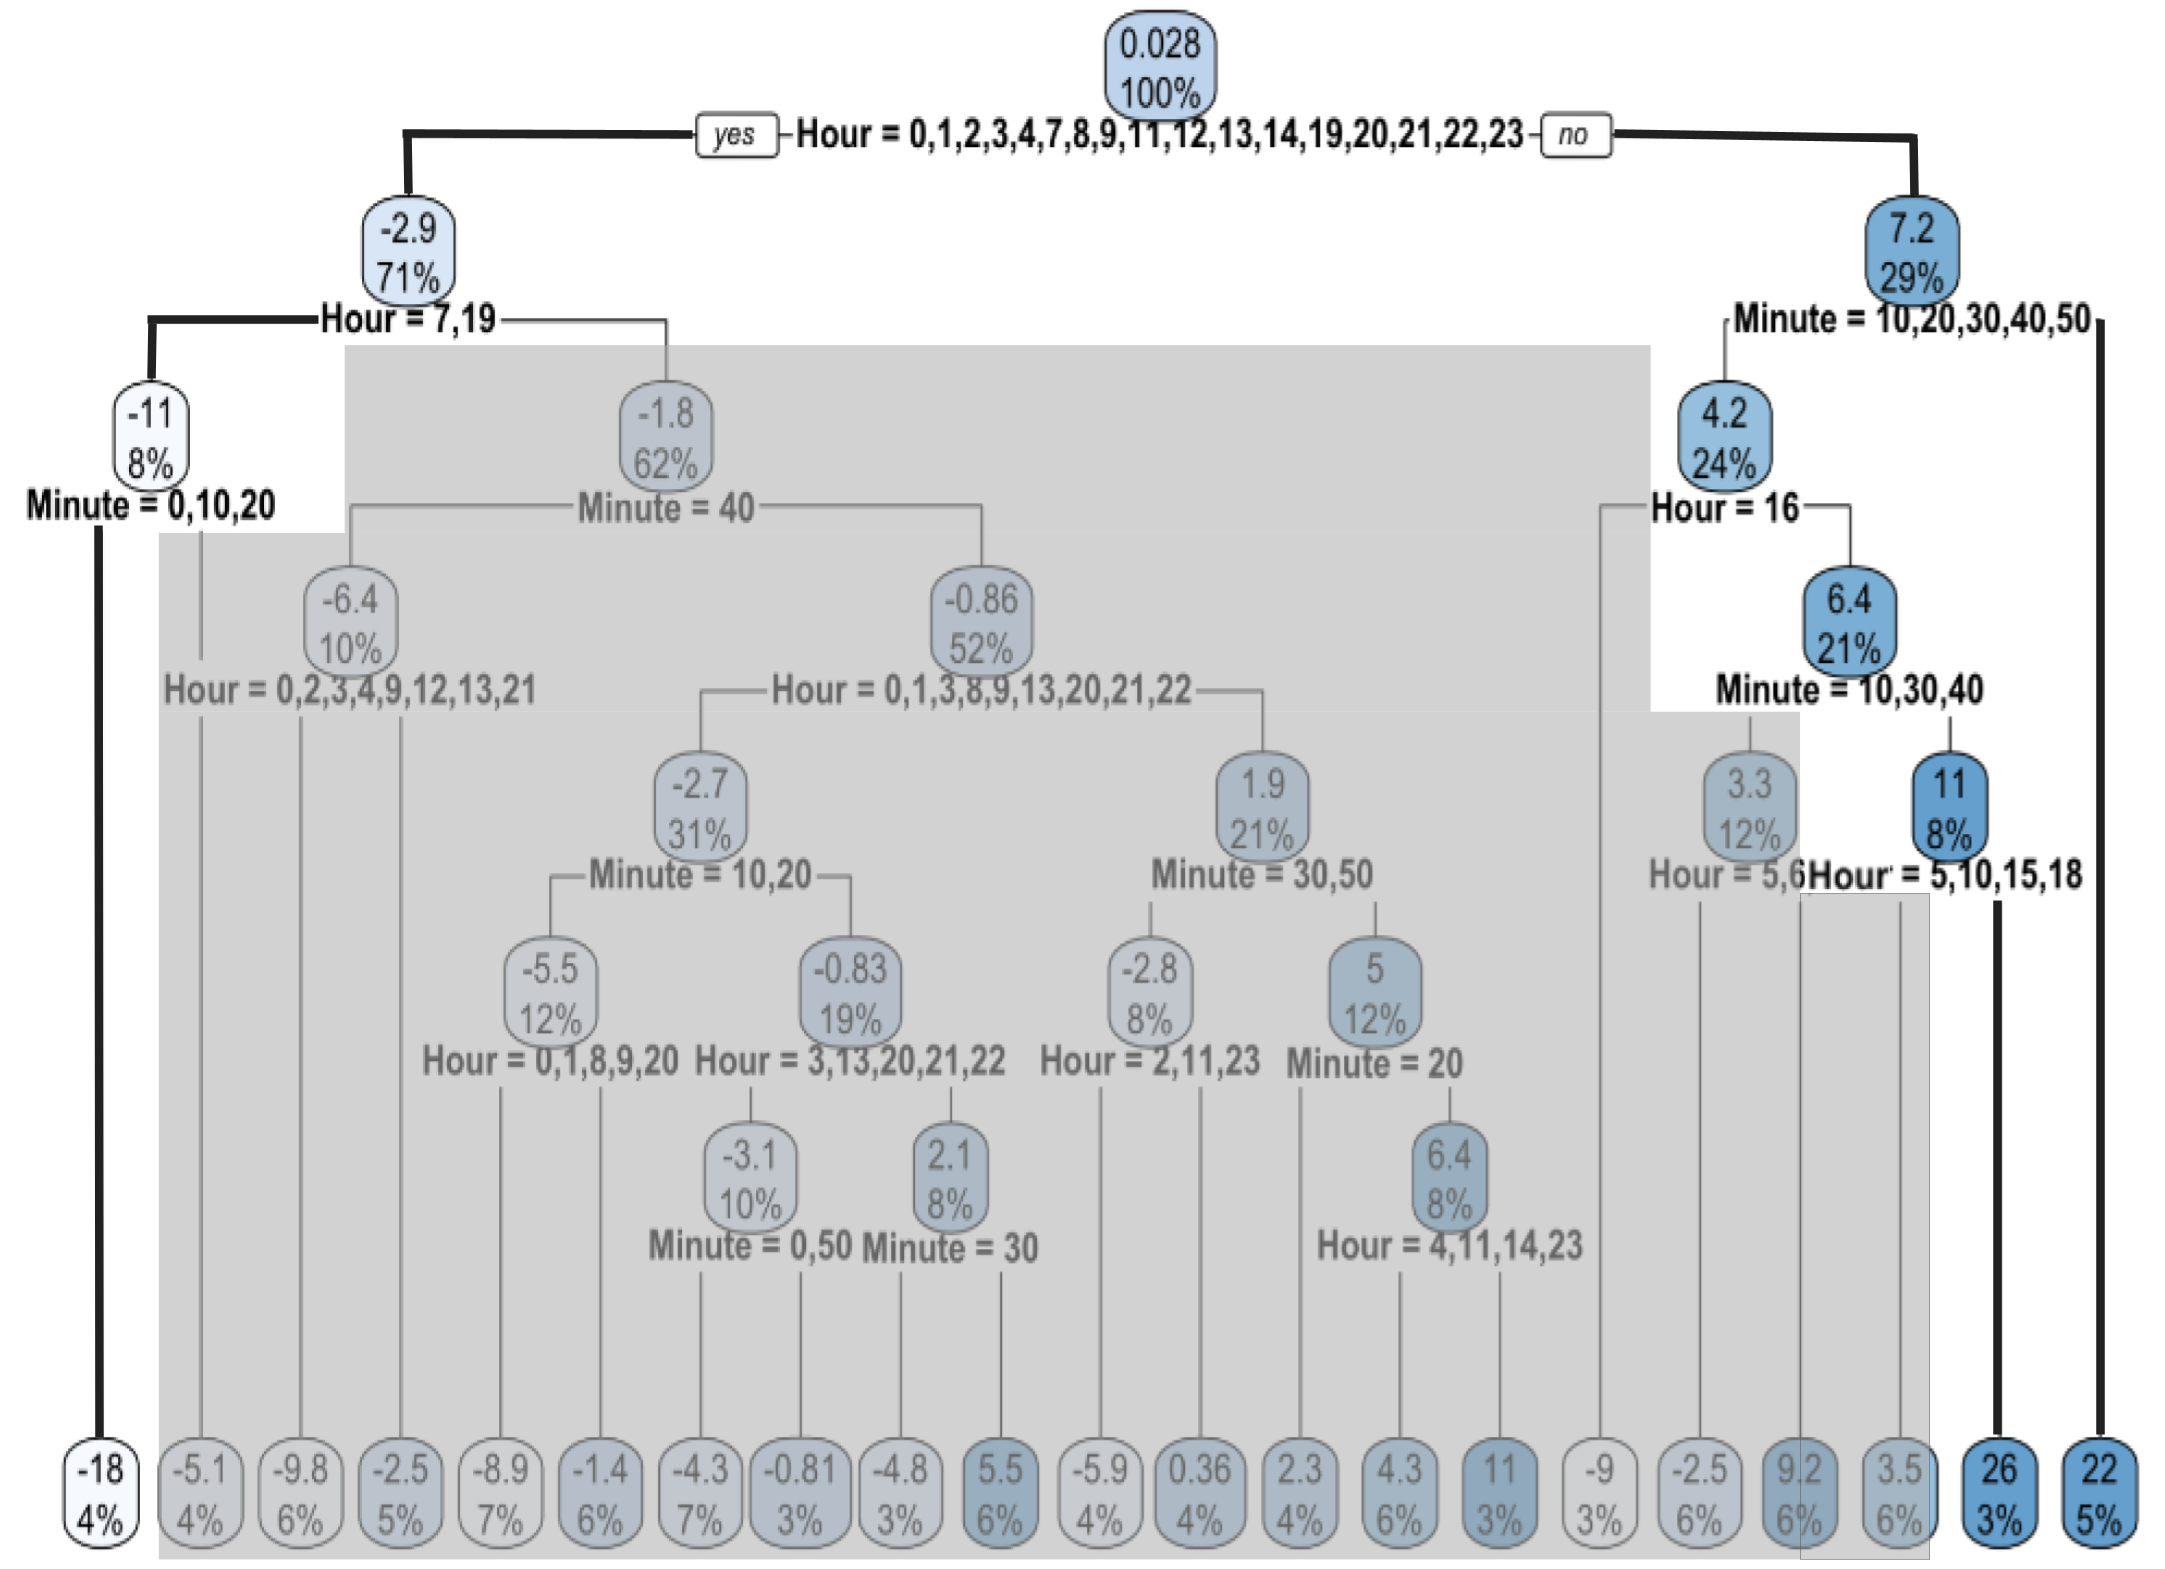
\includegraphics[width=.9\textwidth]{Figures/Hollow Tree.png}
\caption{``Hollowed out'' regression tree of forecast errors.}
\label{fig:tree}
\end{figure}

\FloatBarrier

Determining $k$ requires consideration of lift performance and operational capacity. Increasing $k$ adds terminal nodes with smaller mean error magnitudes. This weakens rule performance and increases the proportion of flagged periods. A large $k$ may be informative for data scientists seeking to identify and remove systematic model bias. For managers, however, acting on flagged periods incurs non-trivial costs in time, attention, and operational effort. Following Shmueli et al.\cite{shmueli2024machine}, we treat $k$ as a resource-constrained ``ranking'' goal rather than a traditional data-driven tuning choice. Managers would choose the smallest $k$ that gives sufficient lift, ensuring that the total number of flagged periods remains within the organization's capacity to act on.

\subsection{Step 5 - Rule Visualization}
\label{subsec-step5}

\matt{Figure~\ref{fig:VizDemo} illustrates TreeAlert's visualization output using three weeks of Luxembourg's electricity demand. The top-$k$ rules ($k$=2) are overlaid on both the actual/forecast series (top panel) and the error series (bottom panel), with flagged periods marked as color-coded circles. Each flagged point in the error panel corresponds to the same period in the series panel. The absence of flagged errors for a particular peak or dip in the error plot may be due to errors not associated with a recurring pattern, a corresponding failure condition whose terminal node's mean error is diluted by non-extreme errors, or missing temporal or contextual predictors that are needed to capture the underlying failure pattern}

\begin{figure}[t!]
  \centering
  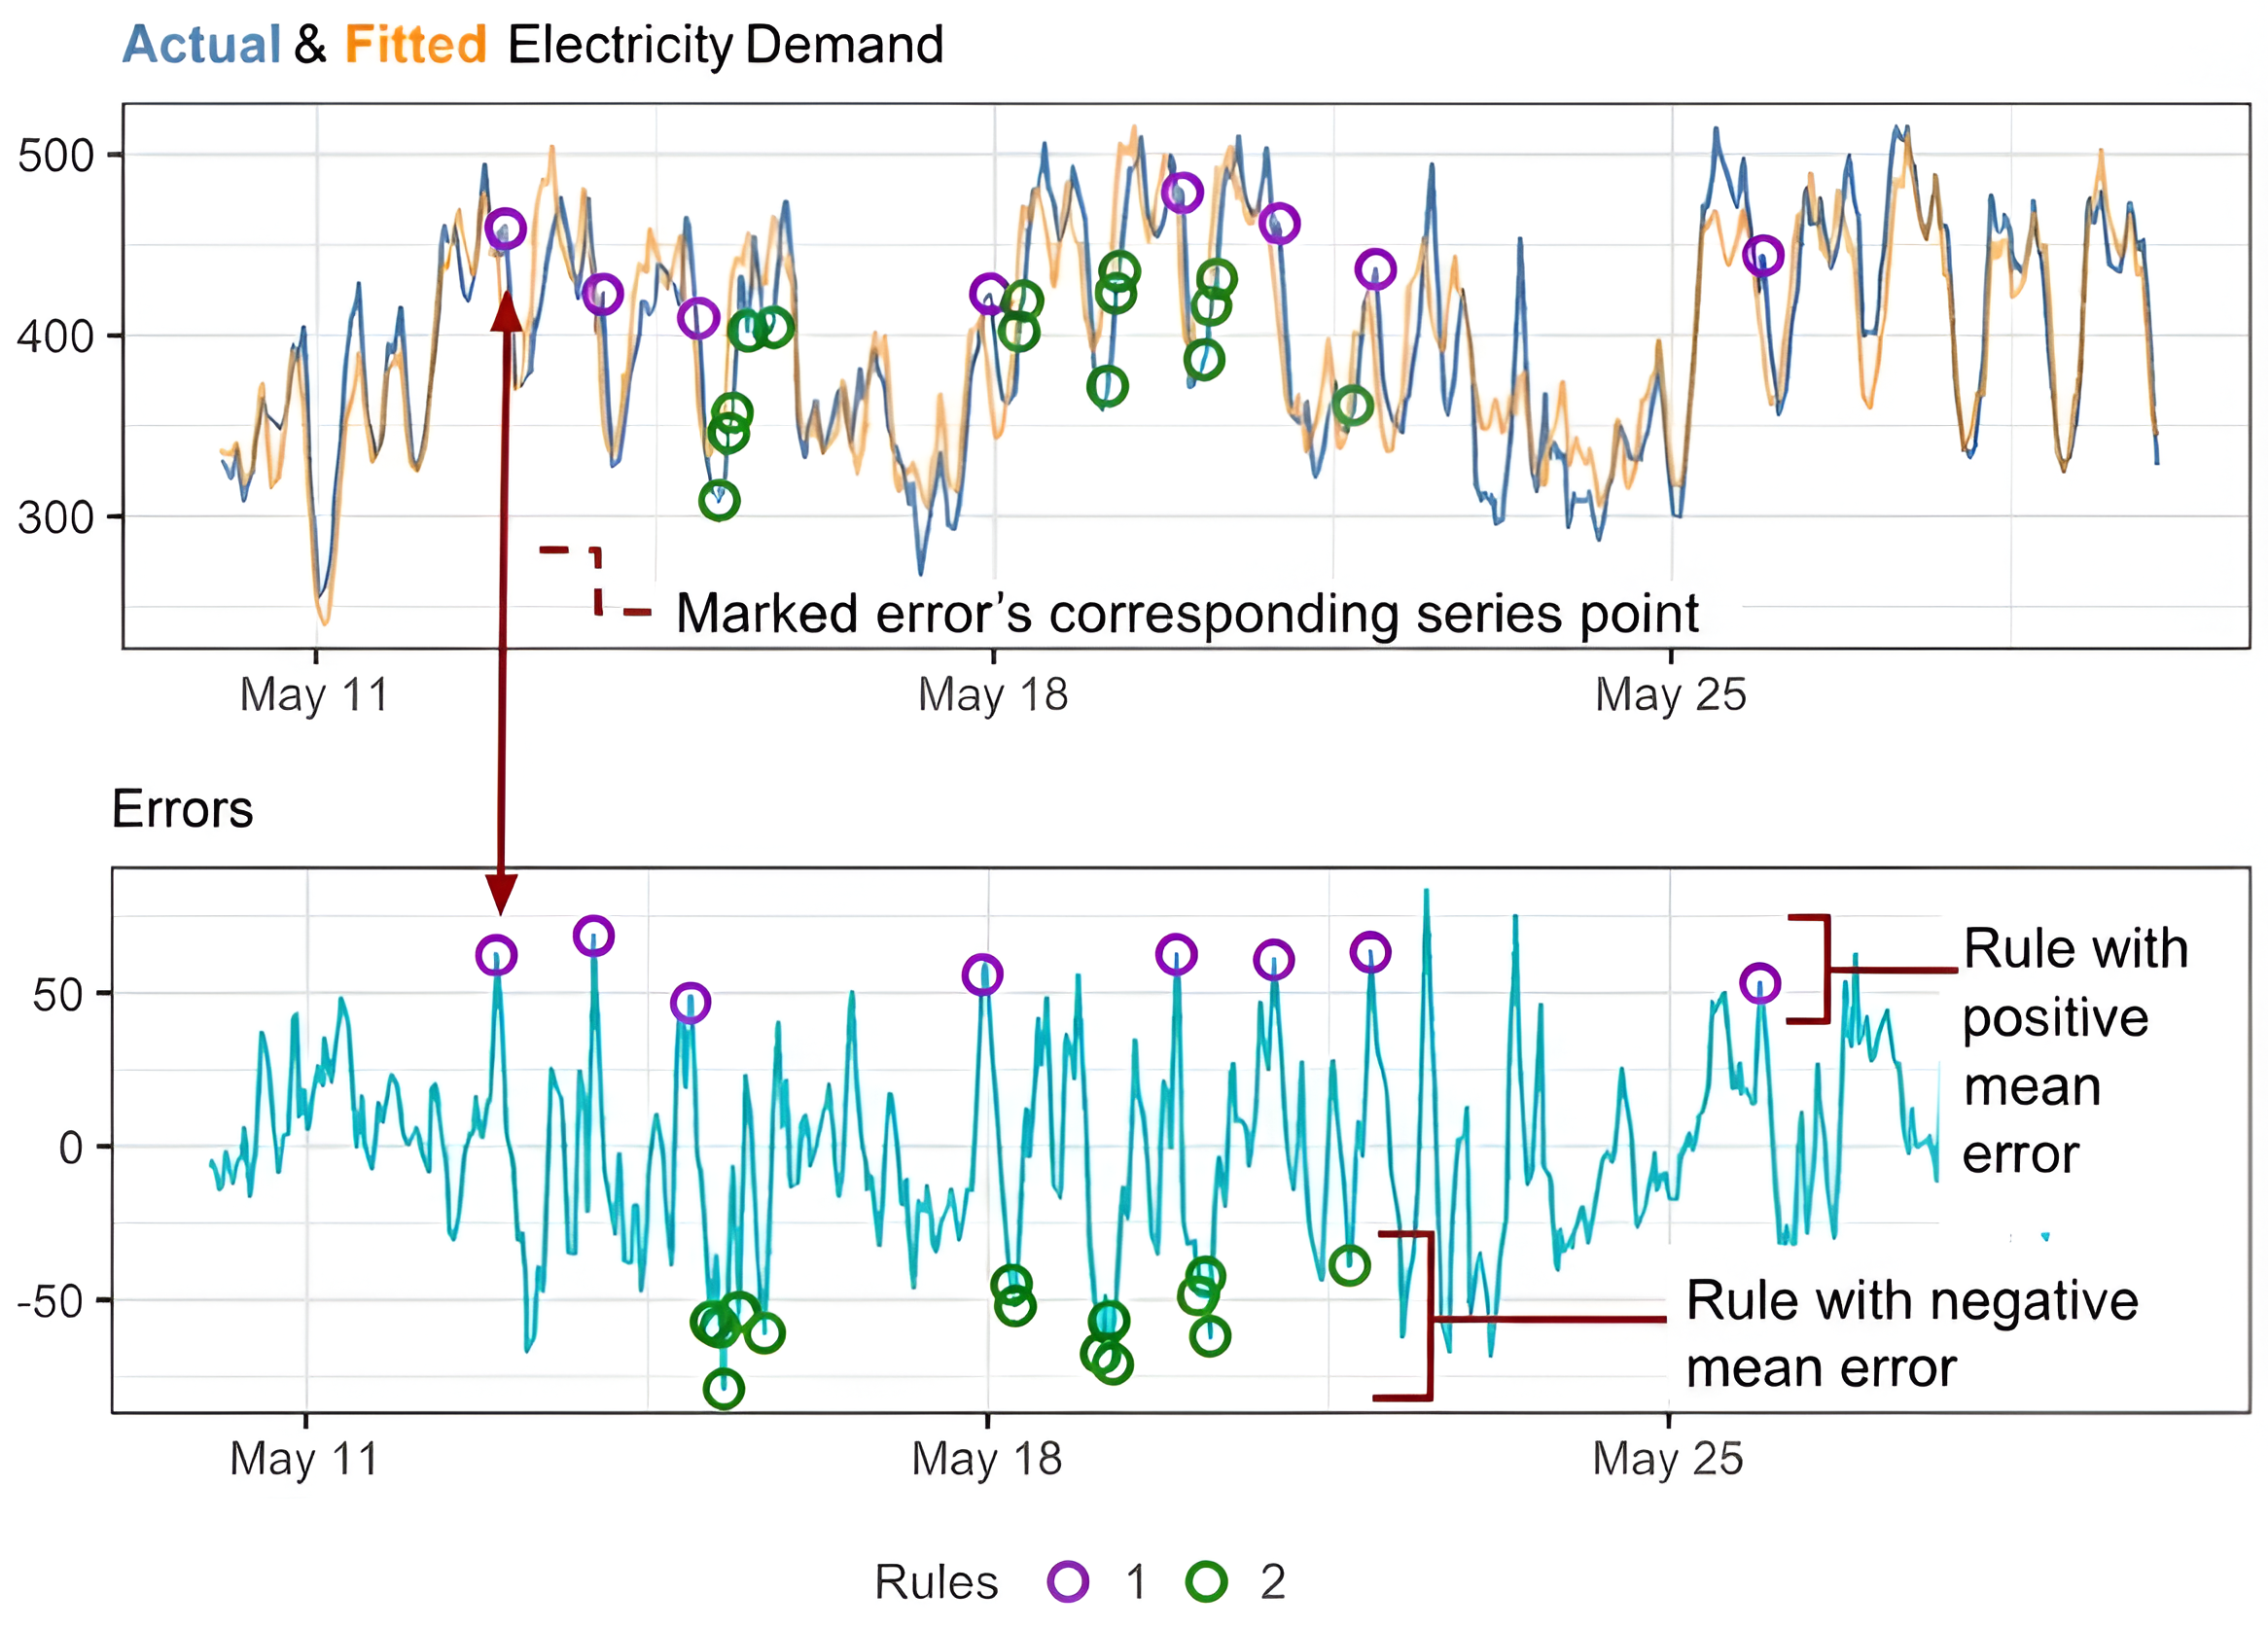
\includegraphics[width=.85\linewidth, trim=0pt 0pt 0pt 0pt, clip]{Figures/VizDemo.png}
  \caption{TreeAlert reveals extreme forecasting failures in Luxembourg's electricity demand model. Negative rule means reflect over-forecasting; positive rule means reflect under-forecasting.}
  \label{fig:VizDemo}
\end{figure}

\subsection{Step 6 - Interpretation}
\matt{We develop a deterministic interpretation module that converts extracted rules (e.g., from \texttt{rpart.rules}) into predictive alerts by aligning rule logic with the data encoding and the algorithm's behavior.\footnote{We also explored LLM-based rephrasing, but found outputs inconsistent, raising concerns about reliability and transparency; we therefore adopt a deterministic procedure.} Extracted rules present three issues. First, rules may overlap because only inclusion conditions are reported, omitting exclusions implied by upstream splits.
For example, consider:}

\begin{itemize}
    \setlength{\itemsep}{0pt}
    \setlength{\parskip}{0pt}
    \setlength{\topsep}{2pt}
    \item[(R1)] \textit{``Mean error = 33.4 when hour is 5 or 16 and DayofWeek is Sun or Mon or Tues''}
    \item[(R2)] \textit{``Mean error = 16.2 when hour is 5 or 16 and DayofWeek is Sun or Mon''}
\end{itemize}

\matt{Inspection of the underlying tree reveals that R1 implicitly includes the exclusion \textit{``DayofWeek is NOT Sun or Mon''}. Our algorithm uses the training data to recover such exclusions, rewriting R1 as \textit{``DayofWeek is Tues''}, thereby producing non-overlapping rules. Second, rule phrasing can hinder interpretation by reflecting observation-level or-conditions rather than the forecasting algorithm's behavior. R2 indicates failures at 5:00 \emph{or} 16:00 on Sunday \emph{or} Monday, but for decision-making should be interpreted as the algorithm being prone to failure at both 5:00 and 16:00 on Sundays and Mondays. Third, predictor values may be misleading without knowledge of the data's temporal resolution. For instance, ``Minute is 10 or 20'' \galit{means} failure over 10--29 minute intervals, not discrete minutes.}

\matt{The module resolves these issues, yielding consistent, non-overlapping, and interpretable rules. We also explored LLM-based rephrasing, but found outputs inconsistent; we therefore adopt a deterministic procedure. Section~\ref{sec-demo} illustrates the resulting rules.}

\subsection{Step 7 - Failure Prediction and Performance Evaluation}

\subsubsection{Failure Prediction}

TreeAlert applies the learned decision rules to an unseen test set. Specifically, it iterates over each future timestamp, checking its correspondence with the $k$ rules learned from the training data. If a future timestamp satisfies the conditions of any rule associated with extreme errors, it is flagged.

\subsubsection{Evaluating TreeAlert's Generated Rules Using Lift}
\label{Sup-A}

Evaluating TreeAlert's predictive performance is essential, as error behavior may differ between training and test sets, causing training-derived rules to produce false alerts on unseen data. This may also result from suboptimal tuning of TreeAlert's parameters or when the training data does not span sufficient periods to identify error patterns. Employing a split-sample training-test approach in Step 2 enables prediction robustness assessments and guides parameter tuning and rule filtering.

As mentioned earlier, traditional forecasting evaluation metrics such as RMSE, MAE, and MAPE, are global performance measures that assess predictive performance across the entire dataset, implicitly assigning equal importance to all time periods. Contrarily, TreeAlert is specifically designed to detect and predict patterns of extreme forecasting failures, which  arise within a subset of temporally and contextually defined periods. Hence, we use lift as our core evaluation metric. Lift is computed separately on the training and test periods, and used to evaluate TreeAlert's ability to capture the subset of most extreme pattern-based failures. We focus on lift in a selected top percentile (e.g., the top ventile) $g_1$. Lift($g_1$) measures the degree to which the alerted subset concentrates extreme errors relative to the entire period. Lift values above 1 indicate better performance of the alerting segment compared to the baseline of no rules (overall MAE). The higher the lift value, the better TreeAlert captures failure patterns compared to treating all periods as equally risky.

While we would have liked to compare TreeAlert's performance against alternative models, we have not been able to identify alternatives aimed at predicting the \emph{timing} of extreme model failures. We bemoan the lack of a fair comparison benchmark, and therefore offer TreeAlert's outputs as a foundational benchmark for this emerging area. We note that for such methods to serve as valid comparators, they should adhere to the eight principles.

\section{Demonstrations of TreeAlert}
\label{sec-demo}

TreeAlert offers actionable insights into critical applications where extreme forecasting
failures can have serious implications. In this section, we present two applications drawn
from distinct domains: electricity demand forecasting and personal health monitoring.
Each application demonstrates TreeAlert's ability  to evaluate a model's forecasts by uncovering patterns characterized by recurring contextual conditions associated with extreme failures. Then, TreeAlert applies the learned patterns to predict future risky periods.

\subsection{Example 1: Forecasting Electricity Demand}

Electricity demand forecasting is critical for grid stability and operational efficiency. Missed forecasts of demand peaks can cause grid stress, price volatility, outages and affect distribution networks \citep{ciarreta2023, gilbert2023, steinbuks2019}. In this application, we use TreeAlert to identify recurring patterns of extreme forecasting errors and predict future failures using electricity demand data from European power systems. Specifically, we apply TreeAlert to four months of 15-minute electricity load demand and the corresponding official operational forecasts for the Germany-Luxembourg bidding zone \citep{entsoe2025}. Data is provided by the Transmission System Operators (TSO), while the specific forecasting models and methodologies used to generate them are not disclosed.
\newline

\noindent\textbf{Step 1 - Feature Engineering:} Derived from the timestamps, we create three temporal predictors: minute-of-hour, hour-of-day, and day-of-week.
\newline

\noindent\textbf{Step 2 - Data Partitioning:} The series is partitioned using a 75/25 split, where the first three months of the data serve as the training set, and the last month is reserved as the test set. This is visualized in Figure \ref{fig:electricity} where the train/test partition is displayed by a red dashed line.
\newline

\noindent\textbf{Step 3 - Regression Tree:} We train a regression tree on the forecast errors as a function of the three temporal predictors. Using lift for hyperparameter tuning, we obtain $n = 5$ and $cp = 0$. These values appear to balance the relatively long series (2,119 periods of 15-min buckets) with many patterns of extreme errors.
\newline

\noindent\textbf{Step 4 - Rule Extraction and Filtering:} \label{sec:rule_filtering}
The top four rules with most extreme average error magnitude are shown in Table \ref{tab:Electricity_Table}.
The positive mean errors across all terminal nodes indicate a systematic bias toward under-forecasting during conditions that lead to extreme errors. We set $k$=4 because $k>4$ introduces terminal nodes with significantly lower
average error magnitudes.
\newline

\begin{table}
\centering
\caption{Top four extreme terminal node rules}
\label{tab:Electricity_Table}
\footnotesize
\renewcommand{\arraystretch}{1.3}
\setlength{\dashlinedash}{2pt}
\setlength{\dashlinegap}{2pt}

\begin{tabular}{|c|m{2cm}|m{10cm}|}
\hline
 & \textbf{Source} & \textbf{Rule} \\
\hline

\multirow{2}{*}{\Large\textcolor{violet}{$\bullet$}}
& Regression Tree Rule
& 4861.59 when Weekday is Sun or Mon \& Hour is 17 or 18 \& Minute is~0 \\
\cdashline{2-3}
& Interpretation
& \textit{The model under forecasts when Weekday is Sunday through Monday, Hours 5PM--6PM and Minute is 0 through 14.} \\
\hline

\multirow{2}{*}{\Large\textcolor[rgb]{0.0,0.6,0.0}{$\bullet$}}
& Regression Tree Rule
& 4041.32 when Weekday is Tue or Wed or Thu or Fri or Sat \& Hour is 17 or 18 or 19 \& Minute is 15 or 30 \\
\cdashline{2-3}
& Interpretation
& \textit{The model under forecasts when Weekday is Tuesday through Saturday, Hours 5PM--7PM and Minute is 15 through 44.} \\
\hline

\multirow{2}{*}{\Large\textcolor{blue}{$\bullet$}}
& Regression Tree Rule
& 5857.96 when Weekday is Sun or Mon or Tue or Wed \& Hour is 2 or 12 \& Minute is 15 or 30 \\
\cdashline{2-3}
& Interpretation
& \textit{The model under forecasts when Weekday is Sunday through Wednesday, Hours 2AM and 12PM and Minute is 15 through 44.} \\
\hline

\multirow{2}{*}{\Large\textcolor{orange}{$\bullet$}}
& Regression Tree Rule
& 3796.82 when Weekday is Sun or Mon \& Hour is 19 \& Minute is 0 \\
\cdashline{2-3}
& Interpretation
& \textit{The model under forecasts when Weekday is Sunday through Monday, Hour 7PM and Minute is 0 through 14.} \\
\hline

\end{tabular}
\end{table}

\begin{figure}[t]
\centering
\caption{\centering Electricity demand, forecasts, and forecast errors, with TreeAlert's flagged periods}
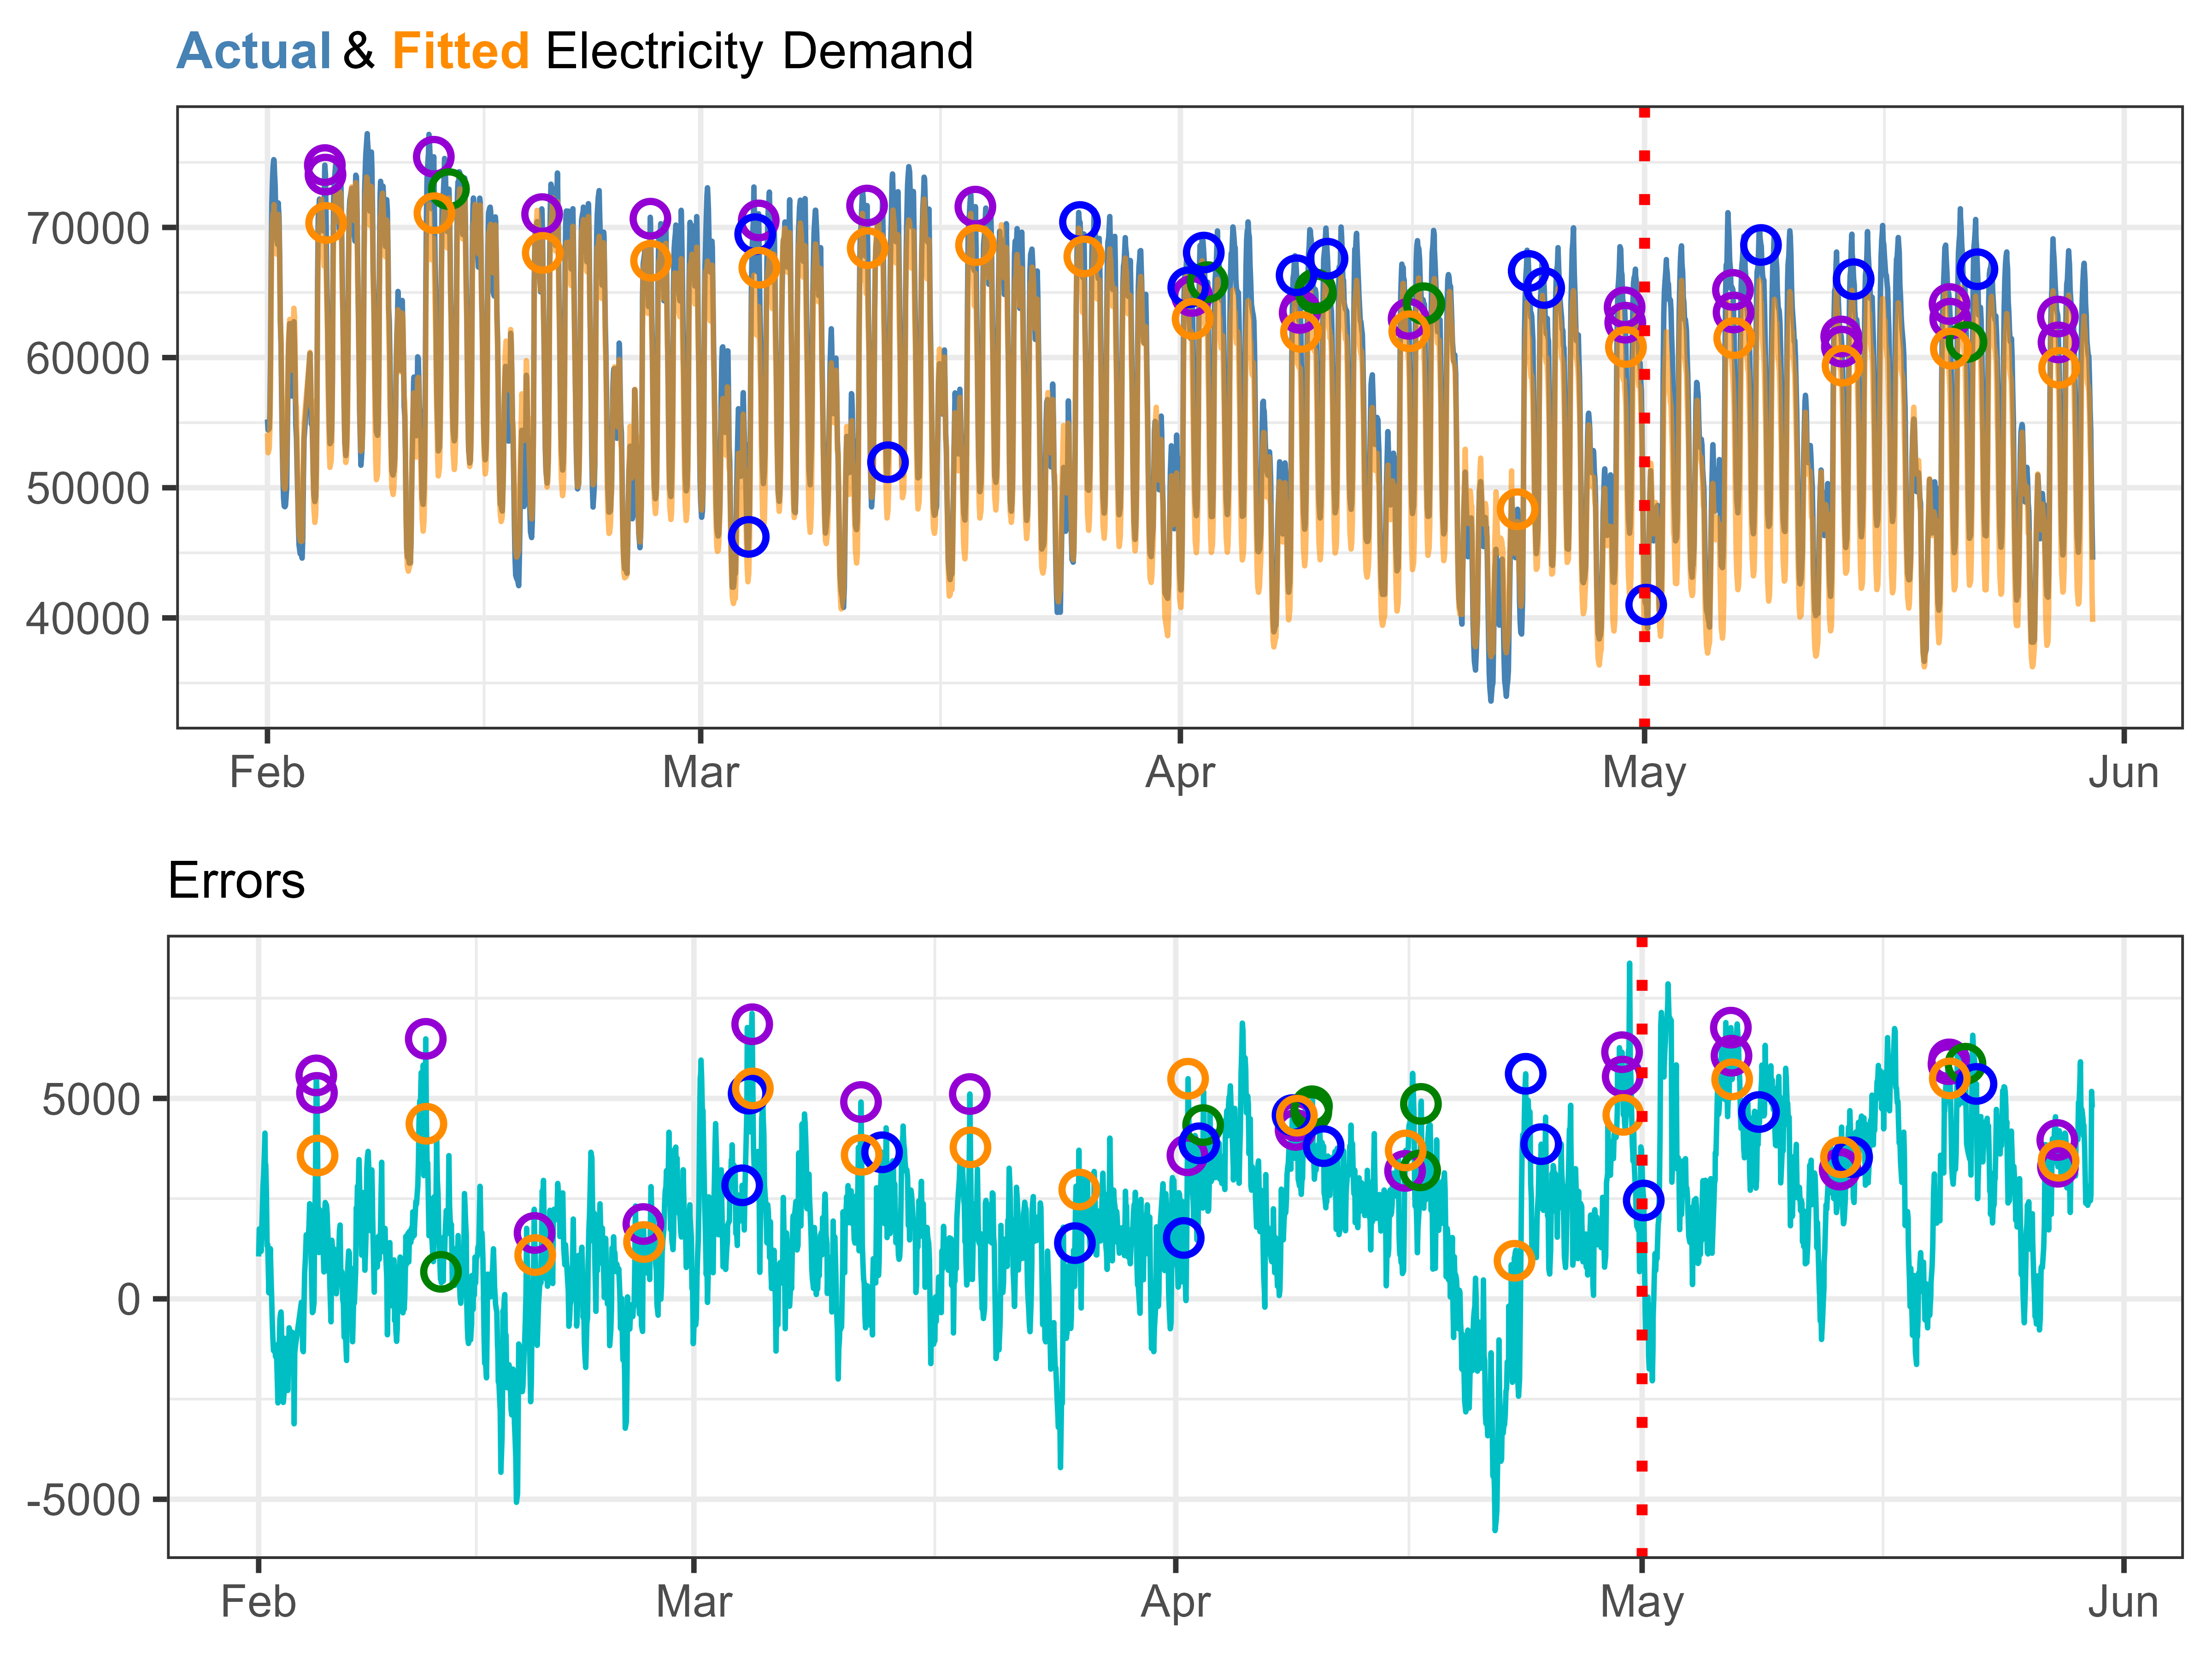
\includegraphics[width=.9\textwidth]{Figures/Electricity.png}
\label{fig:electricity}
\end{figure}

We note that patterns of extreme failure due to dips in the error series (over-forecasts) are not flagged in this example because their terminal nodes did not yield a sufficiently high mean error to rank among the top-$k$ rules. However, to also flag common patterns of over-forecasted periods, we can adjust Step~4 (Rule Extraction and Filtering) to retain the top $k_1$ negative and $k_2$ positive mean error rules; see example in Supplemental Material 4.
\clearpage

\noindent\textbf{Step 6 - Interpretation:}
Each resulting rule is translated using the interpretation module (see Table \ref{tab:Electricity_Table}). The translated rules indicate under-forecasting of electricity demand during early evening hours, especially from Sunday to midweek. These flagged periods align with demand peaks in Figure \ref{fig:electricity}, suggesting that the errors stem from increased electricity demand during these periods. These insights help decision makers anticipate times when forecasts are unreliable and guide algorithm designers in improving model performance under such conditions.
\newline

\noindent\textbf{Step 7 - Evaluating Predictive Performance:} \matt{Table~\ref{tab:elec_performance} summarizes predictive performance across  training and test sets. Figures~\ref{fig:elec_lift_test} present a ventile lift charts using 20 equal-sized groups. The test lift of 1.32 confirms that flagged periods concentrate errors approximately 32\% above the global average. The close alignment between training and test lift indicates that the identified patterns generalize out-of-sample.}

\begin{table}
\tbl{TreeAlert predictive performance -- electricity demand}
{\begin{tabular}{lcccc} \toprule
\textbf{Set} & \textbf{Flagged Periods} & \textbf{Total Periods} & \textbf{\% Flagged} & \textbf{First-ventile lift} \\
\midrule
Training & 33 & 2,119 & 1.6\% & 1.74 \\
Test     & 16 & 696   & 2.3\% & 1.32 \\
\bottomrule
\end{tabular}}
\label{tab:elec_performance}
\end{table}

\begin{figure}[H]
  \centering
  \begin{minipage}{0.39\linewidth}
    \centering
    \includegraphics[width=\linewidth]{Figures/Electricity_Lift_Train.png}
  \end{minipage}
  \hfill
  \begin{minipage}{0.39\linewidth}
    \centering
    \includegraphics[width=\linewidth]{Figures/Electricity_Lift_Test.png}
  \end{minipage}
    \caption{Lift chart for electricity training data (left) and test data (right)}
    \label{fig:elec_lift_test}
\end{figure}

\FloatBarrier
\subsection{Example 2: Forecasting Heart Rate}
\label{subsec:heartrate}

Consider the now ubiquitous health-related smart devices and sensors that collect data on our behaviors, bodies, and environment. Extreme over- or under-forecasts can be dangerous in health monitoring. For example, an IoT device that algorithmically forecasts heart-rate over time exhibits routine fluctuations, but steep peaks and/or dips in heart rate can be indicative of critical health events, necessitating precise and reliable forecasts of these events. We demonstrate the use of TreeAlert to detect extreme failure patterns. Specifically, TreeAlert is applied to forecasts  generated using an ARIMA(4,0,0)(2,0,0)[6] model.  The data is obtained from an IoT-based heart rate monitoring device that recorded heart rate measurements at 10-minute intervals over a two-month period \citep{furberg2016}.
\newline

\noindent\textbf{Step 1 - Feature Engineering:}
We extract three temporal predictors: day-of-week, hour-of-day, and minute-of-hour. In this demonstration we also include two contextual predictors: intensity and steps. Intensity is an ordinal categorical variable measuring the intensity of activity of the device wearer on a scale of 1-3. Steps is the number of steps taken, recorded in each 10-minute interval.
\newline

\noindent\textbf{Step 2 - Data Partitioning:}
We split the heart rate series into the first 3,240 10-min buckets (training) and final 572 buckets (test), yielding a 85/15 temporal train-test split.
\newline

\noindent\textbf{Step 3 - Regression Tree:}
The regression tree is trained on the forecast errors as a function of the three temporal predictors and two contextual predictors. Using lift for hyperparameter tuning, we obtain  $n = 9$ and $cp = 0$.
\newline

\noindent\textbf{Step 4 - Rule Extraction and Filtering:}
\matt{We extract the top three rules (Table \ref{tab:HeartRate_Table}). All corresponding terminal nodes have positive mean errors, indicating systematic under-forecasting. We set $k=3$ to balance rule strength and the number of flagged periods.}
\newline

\noindent\textbf{Step 5 - Rule Visualization:}
\matt{Figure \ref{fig:hr_viz} plots, heart rate values, forecasts and the forecast errors. Each panel highlights periods flagged by the top four rules. Points where rules overlap signal less unreliable periods, where failure conditions converge.}
\newline

\noindent\textbf{Step 6 - Interpretation:}
Table \ref{tab:HeartRate_Table} presents the translated rules revealing model failures during early weekday mornings and late afternoons. These  periods coincide with timings of increased physical activity as all three rules include Steps as a predictor. The Intensity predictor is excluded, likely due to its redundancy with the more granular Steps variable.

\noindent\textbf{Step 7 - Evaluating Predictive Performance:}
\matt{Table~\ref{tab:hr_performance} summarizes predictive performance across training and test sets, with lift computed over 20 equal-sized ventile  groups (Figure~\ref{fig:hr_lift_train}). The test lift of 2.79 indicates
that flagged periods concentrate errors nearly three times the global average. The slightly higher test lift relative to training confirms that the identified failure patterns generalize out-of-sample.}
\begin{table}[b]
\tbl{Top three extreme terminal node rules}
{\footnotesize
\renewcommand{\arraystretch}{1.3}
\setlength{\dashlinedash}{2pt}
\setlength{\dashlinegap}{2pt}
\begin{tabular}{|c|m{2cm}|m{10cm}|}
\hline
 & \textbf{Source} & \textbf{Rule} \\
\hline
\multirow{2}{*}{\Large\textcolor{violet}{$\bullet$}}
& Regression Tree Rule
& 43.73 when Steps\_10 is 466 to 663 \& Hour is 3 or 5 or 10 or 15 or 16\newline or 23 \& Minute is 10 or 20 or 40 or 50 \\
\cdashline{2-3}
& Interpretation
& \textit{The model under forecasts by an average of 44 when Steps\_10 is 466 to 663, Hour is 3AM, 5AM, 10AM, 3PM--4PM, and 11PM, and Minute is 10 through 29 and 40 through 59.} \\
\hline
\multirow{2}{*}{\Large\textcolor[rgb]{0.0,0.6,0.0}{$\bullet$}}
& Regression Tree Rule
& 39.79 when Steps $\geq$ 1018 \& Hour is 4, 6--9, 11--13, 16--22 \\
\cdashline{2-3}
& Interpretation
& \textit{The model under forecasts by an average of 35 when Steps $\geq$ 1018 and Hour is 4AM, 6AM--9AM, 11AM--2PM, and 5PM--10PM.} \\
\hline
\multirow{2}{*}{\Large\textcolor{blue}{$\bullet$}}
& Regression Tree Rule
& 30.91 when Steps is 523 to 1018 \& Hour is 7 or 8 or 11 or 13 or 14 or 17 \& Minute is 20 or 40 or 50 \\
\cdashline{2-3}
& Interpretation
& \textit{The model under forecasts by an average of 30 when Steps is 523 to 1018, Hour is 7AM--8AM, 11AM, 1PM--2PM, 5PM, and Minute is 20 through 29 and 40 through 59.} \\
\hline
\end{tabular}}
\label{tab:HeartRate_Table}
\end{table}

\begin{figure}[H]
  \centering
  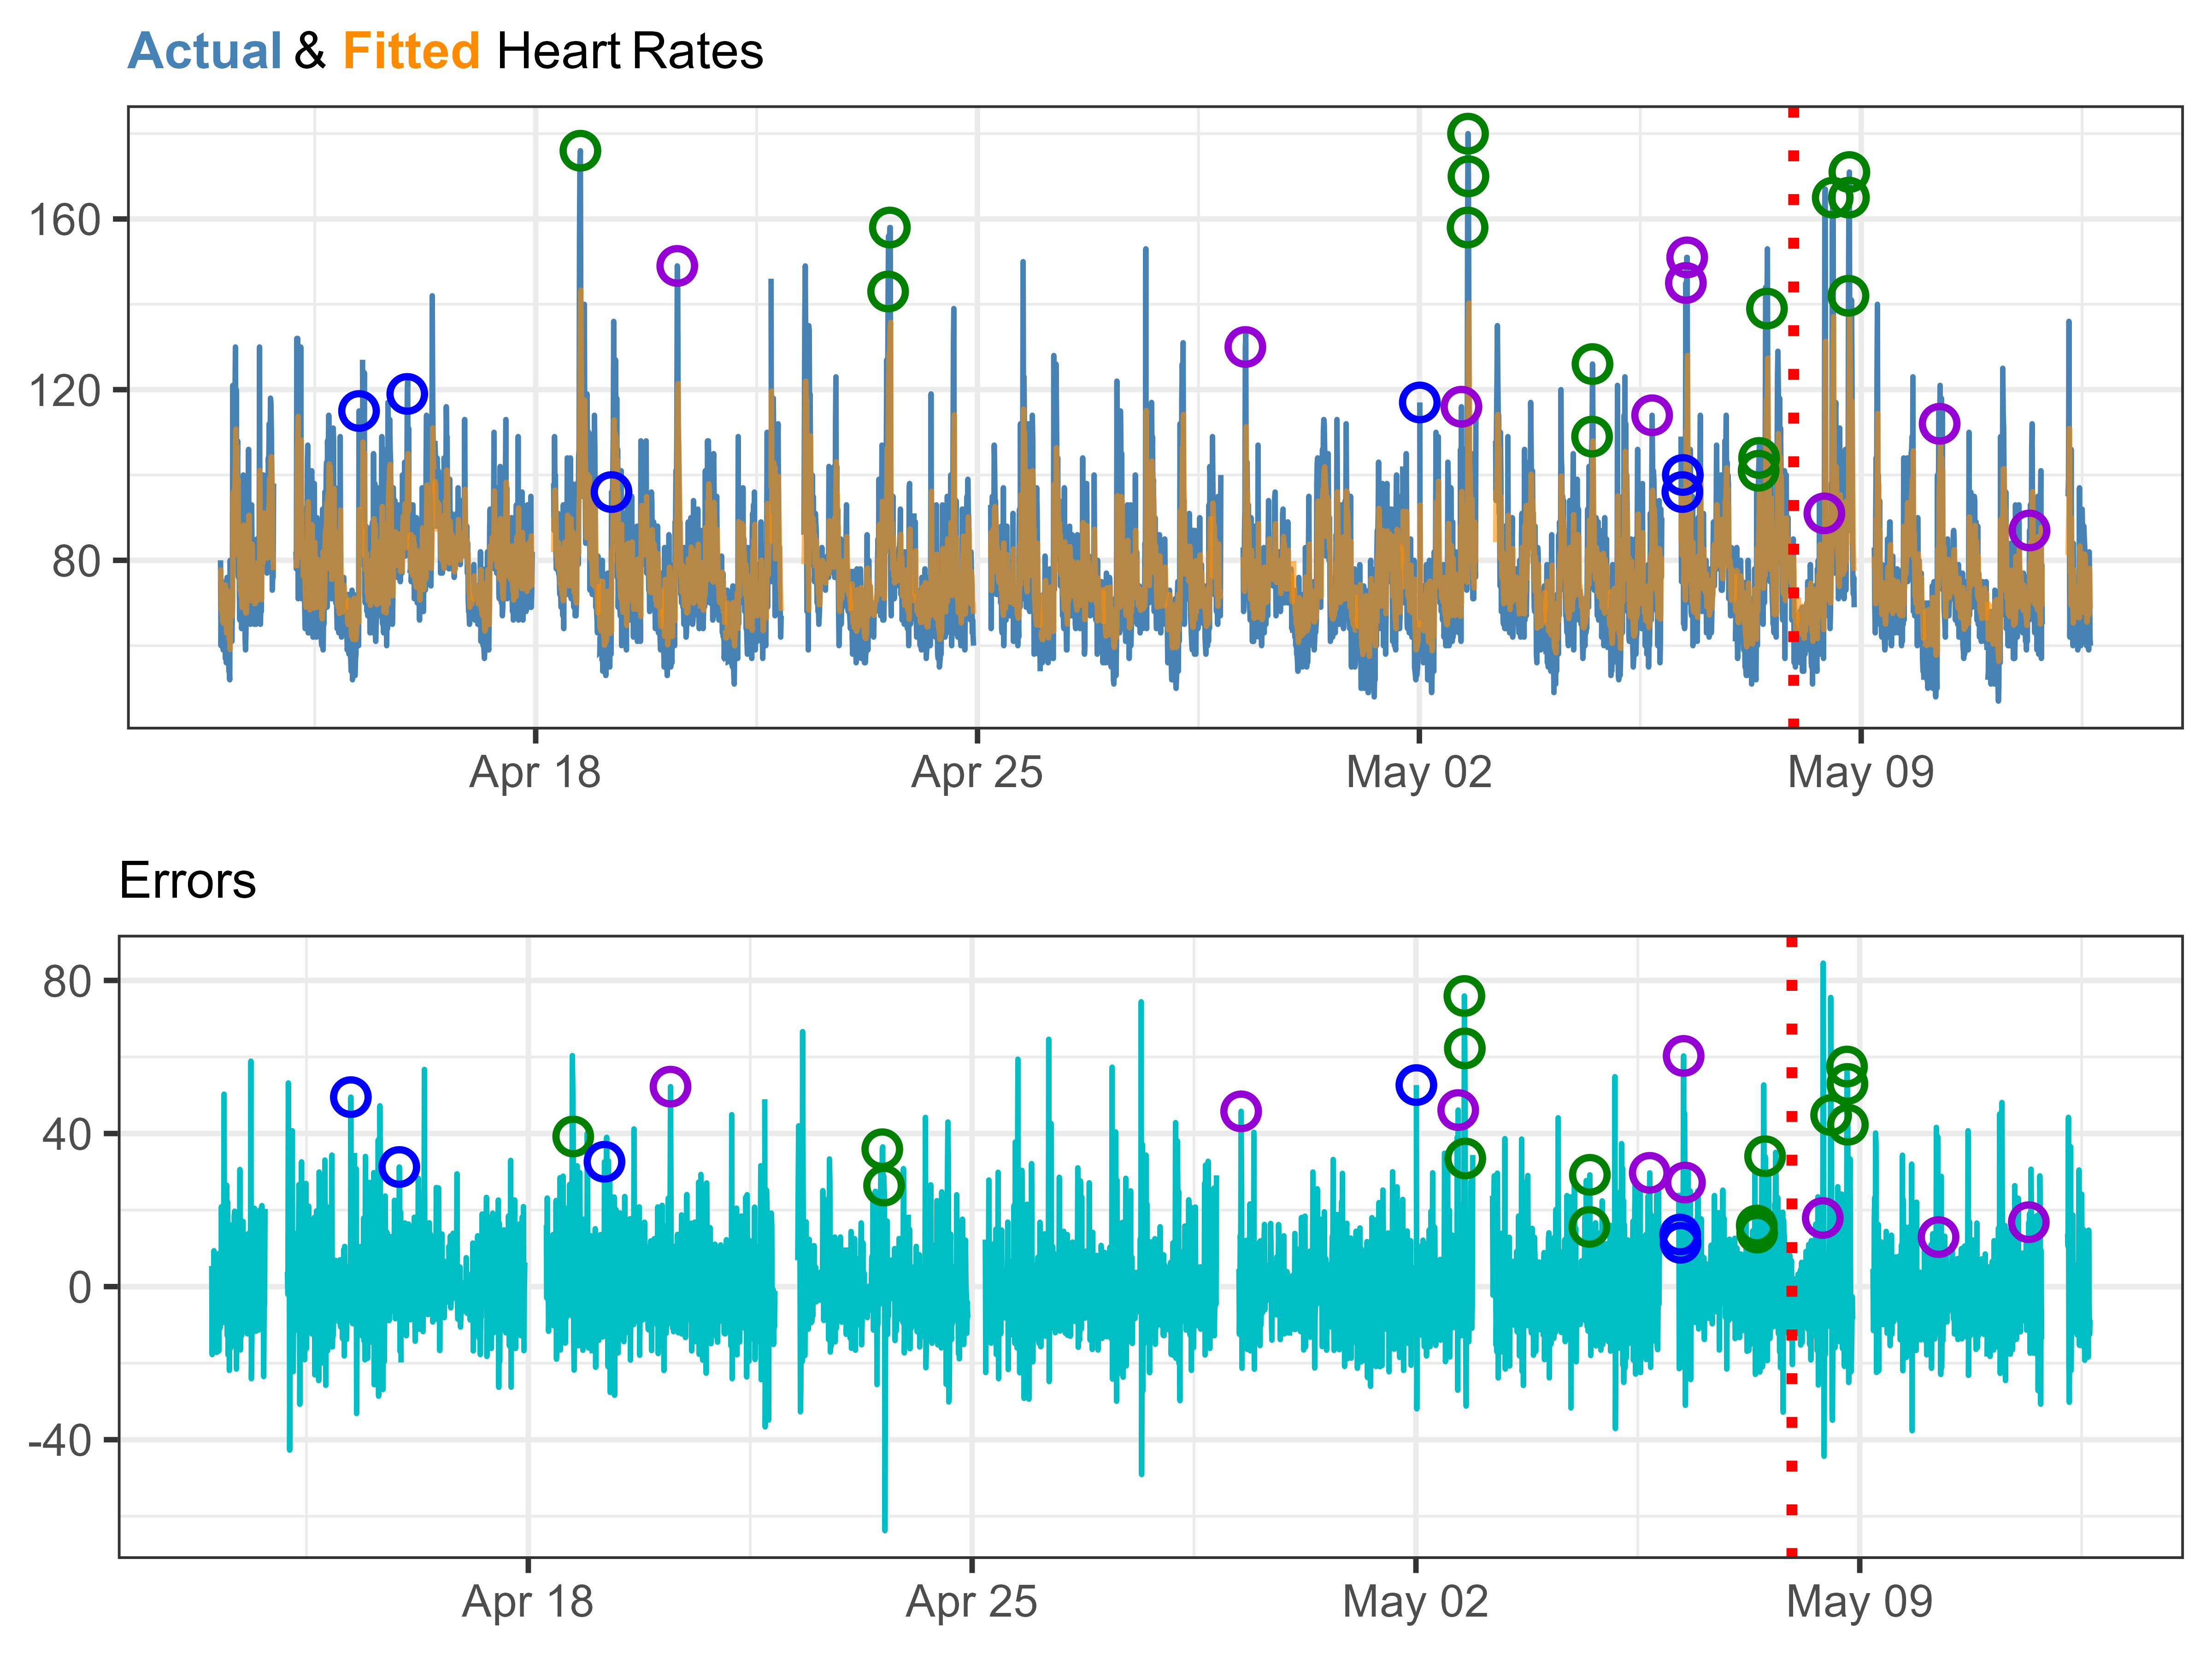
\includegraphics[width=.9\textwidth]{Figures/hr_viz.png}
  \caption{Heart rate, forecasts, and forecast errors series, with TreeAlert's flagged periods}
  \label{fig:hr_viz}
\end{figure}

\FloatBarrier

\newline

\begin{table}
\tbl{TreeAlert predictive performance -- heart rate}
{\begin{tabular}{lcccc} \toprule
\textbf{Set} & \textbf{Flagged Periods} & \textbf{Total Periods} & \textbf{\% Flagged} & \textbf{First-ventile lift} \\
\midrule
Training & 55 & 3,240 & 1.7\% & 2.62 \\
Test     & 12 & 572   & 2.1\% & 2.79 \\
\bottomrule
\end{tabular}}
\label{tab:hr_performance}
\end{table}

\begin{figure}[H]
  \centering
  \begin{minipage}{0.4\linewidth}
    \centering
    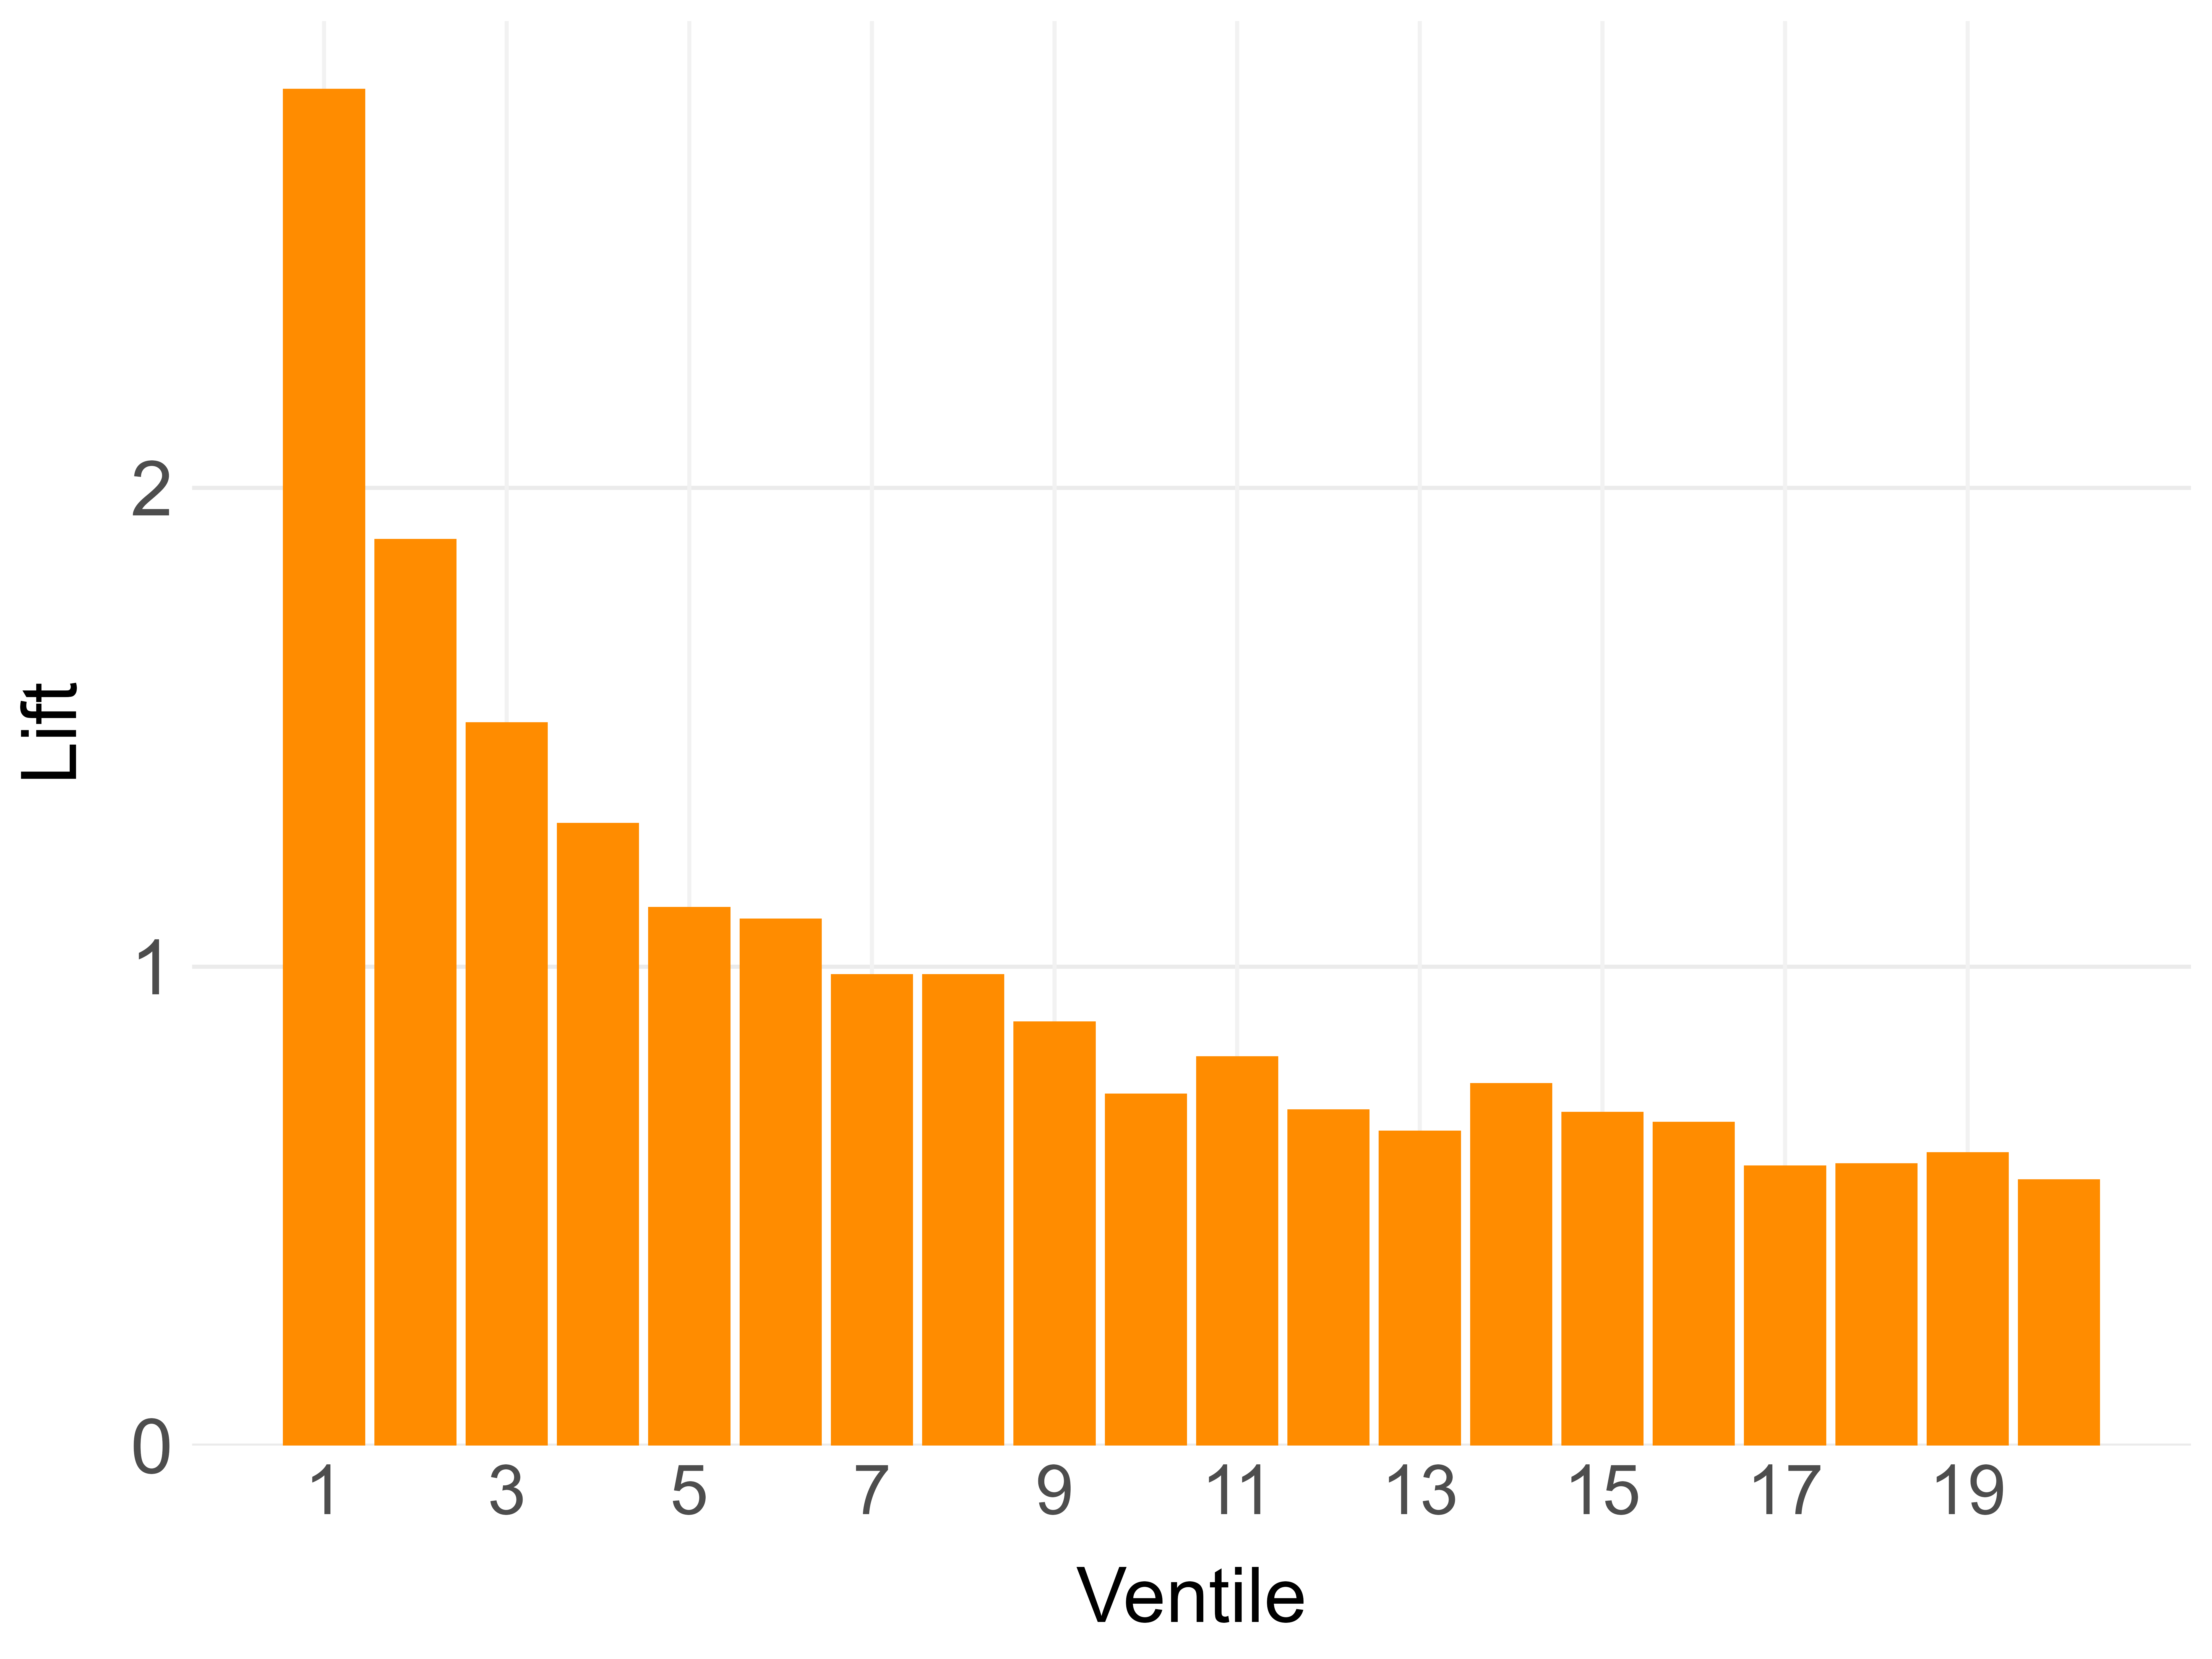
\includegraphics[width=\linewidth]{Figures/HR_Lift_Train.png}
  \end{minipage}
  \hfill
  \begin{minipage}{0.4\linewidth}
    \centering
    \includegraphics[width=\linewidth]{Figures/HR_Lift_Test.png}
  \end{minipage}
    \caption{Lift chart for heart rate data (left) and test data (right)}
    \label{fig:hr_lift_train}
\end{figure}

\FloatBarrier
\section{Discussion}

Extreme failures of time-series forecasts are sudden shocks to predictive systems that underlie major financial, health, and other critical services. Traditional error analysis is blind to these sudden events and cannot guide practitioners anticipate or avoid \galit{them}. Handling extreme failures requires a rethink in how we conceptualize, detect, and describe patterns of disparate but related \galit{forecast failures}. To these ends, we developed TreeAlert as a general method for detecting extreme failure patterns of time series forecasting algorithms that \galit{are} used to predict the timing of future failures. By proactively identifying extreme failure patterns, predicting periods of extreme failures, and offering understandable description of these patterns, TreeAlert can be practically valuable in a wide range of applications including digital platforms, electronic markets, fintech, and other domains where acting on, or ignoring, extreme failures \galit{has} serious ramifications.

Beyond practical value, we \galit{offer} methodological contributions by \galit{integrating and adapting statistical and machine learning methods}
in strategic, new configurations. We extend the machine learning area of error analysis to the domain of time series forecasting in a few novel ways. First, whereas conventional error analysis focuses on classifying a binary outcome as a function of a dataset's features (e.g., Microsoft's Azure error analysis tool),
we model the relationship between a numeric forecast error and specially-constructed
temporal and contextual features. Second, rather than weighting all errors uniformly, we target only the most extreme errors using a specialized pruning technique that isolates outer tree branches, and evaluate performance using a lift metric that assesses the model's ability to concentrate the most extreme errors within the highest-ranked predictions. Third, we move beyond retrospective error diagnostics by generating interpretable decision rules that predict the timing \galit{and} context of future model failures.

Our choice of regression trees as the basis of TreeAlert is critical to adhere to our eight principles. We selected regression trees for their balance of interpretability, efficiency, and predictive capability. Such trees automatically identify informative predictor combinations and group similar error magnitudes (\emph{P6: Local Performance}). Critically, their interpretable rule-based outputs clearly outline conditions of forecasting errors, enabling TreeAlert to predict extreme failure patterns (\emph{P1: Pattern-focus}; \emph{P5: Prospective}) with actionable, decision-maker-ready insights (\emph{P2: Actionability)}. Blackbox models, by contrast, obscure feature interactions and are ill-suited to settings requiring integrating external judgment with risk assessment or explainability \citep{rudin2019, houssainy2021}, undermining \emph{P4: Transparency}. Post-hoc approximations such as SHAP and LIME do not faithfully represent true internal behavior \citep{rudin2019} and fail to yield grouped, predictor-combination rules. Furthermore, from only numerical error magnitudes, their timestamps, and potential contextual information, regression trees are able to capture a diverse range of error patterns (P3) with minimal user input to make TreeAlert truly model-agnostic (P7).\footnote{We also investigated classifying errors into ``extreme/non-extreme'' and using classification trees \galit{but met} challenges. First, labeling each error as ``extreme'' or ``non-extreme'' requires a domain-based or statistical rule that is often arbitrary or hard to obtain. Second, dichotomization causes information loss by discarding error magnitudes; the resulting tree cannot group errors with similar magnitudes near label boundaries. Third, terminal nodes are no longer ordered, leading to redundant, partially overlapping rules.}
Our method can be easily extended to support alternative regression tree algorithms, different lengths of series, encompassing different trends, patterns, and seasonal structures.

We balance coverage of diverse extreme conditions with rule specificity by automatically tuning TreeAlert's hyperparameters using lift on a held-out test set. In terms of feature generation, the number and granularity of temporal predictors influence the nature of resulting rules. Too few predictors yield overly broad rules that blur distinct failure conditions, whereas overly fine-grained or high-cardinality predictors can produce highly localized rules that generalize poorly. Temporal predictors should therefore be selected to match the frequency and duration of the time series under study. Finally, the diversity of identified patterns can be further adjusted by the user by modifying the set of temporal features and by increasing/decreasing the number of rules ($k$). For example, as illustrated in Figure~\ref{fig:electricity}, learned rules may emphasize periods of extreme errors concentrated around peaks and dips, while capturing fewer failure patterns outside these periods. In this case, to further capture patterns during non-peaks/dips, we could increase the number of rules.

We also ensured operational integrability (P8) by designing TreeAlert to be generalizable across statistical and machine learning software and seamlessly integrable into automated forecasting systems, such as Meta's Prophet, which are prone to extreme errors during steep peaks and dips. By introducing forward-looking risk assessment through error analysis, TreeAlert transform FSSs into more transparent, actionable, and trustworthy decision-making tools. Moreover, in terms of sustainability, regression trees consume substantially less energy than neural networks.

Finally, in terms of generalizability, as a machine learning model, TreeAlert assumes that the error distribution and the identified failure patterns will remain stable in the future. Hence, changes in the forecasting model's behavior or the data-generating processes can shift the error distribution and reduce the relevance of previously learned rules. Periodic retraining on recent forecast errors, as well as adaptive or sliding-window extensions, offer promising directions for addressing non-stationary error dynamics.

\begin{table}
\tbl{TreeAlert Embodies the Design Principles for Pattern-Based Error Prediction}
{\begin{tabular}{p{0.6cm}p{2cm}p{10cm}} \toprule
\textit{P1} & \textit{Pattern-focus} & Uncover patterns of model failure. \\
\textit{P2} & \textit{Actionability} & Outputs interpretable, human-readable rules that managers can use to mitigate risk and data scientists can use for model improvement. \\
\textit{P3} & \textit{Diverse Error Patterns} & Accommodates a wide range of extreme error sources such as steep peaks, sparse data, misaligned seasonality, and slow model adjustment. \\
\textit{P4} & \textit{Transparency} & Produces a transparent, interpretable rule-based output. \\
\textit{P5} & \textit{Prospective} & Predicts the future timing and context of potential model failures. \\
\textit{P6} & \textit{Local \newline Performance} & Evaluation focuses on local performance using lift-based ranking. \\
\textit{P7} & \textit{Model-agnostic} & Operates on forecast errors from any forecasting algorithm. Its design does not rely on model-specific assumptions, making it adaptable across methodologies and software platforms. \\
\textit{P8} & \textit{Operational \newline Integrability} & Operationally efficient at every modeling stage: parsimonious inputs, low training overhead via regression trees, and simple deployable rules that integrate seamlessly into existing forecasting systems and dashboards. \\
\bottomrule
\end{tabular}}
\label{tab:design}
\end{table}

Our eight principles are a substantial contribution in their own right, and should guide the development of future methods for predicting patterns of extreme failures. Table~\ref{tab:design} summarizes how TreeAlert aligns with these principles, highlighting its practical and theoretical contributions to pattern-based error prediction. Rather than relying on ad-hoc approaches centered on accuracy metrics or retrospective diagnostics, our framework prioritizes identifying error patterns, interpretable outputs, and operational relevance. These principles guide the design of methods aimed not only at detection but also anticipation and intervention. Our formalization should enable more systematic development of error analysis techniques that are both practical and theoretically grounded.


%%%%%%%%%%%%%%%%%%%%%%%%%%%%%%%%%%%%%%%%%%%%%%%%%%%%%%%%%%%%%%%%%%%%%%%%%%%%%%
%  ACKNOWLEDGEMENTS AND FUNDING
%%%%%%%%%%%%%%%%%%%%%%%%%%%%%%%%%%%%%%%%%%%%%%%%%%%%%%%%%%%%%%%%%%%%%%%%%%%%%%

%\section*{Acknowledgement(s)}

%We extend our sincere gratitude to Ta-Chun Kuan and Carolin Su for their contributions to the development of this research. Original data sources are cited in the references. R code and data reproducing the analyses is available from the first author's Github.

%\section*{Funding}

%This research is partially funded by The National Science \& Technology Council (NSTC), Taiwan, research grant 114-2410-H-007-092-MY3.

%%%%%%%%%%%%%%%%%%%%%%%%%%%%%%%%%%%%%%%%%%%%%%%%%%%%%%%%%%%%%%%%%%%%%%%%%%%%%%
%  REFERENCES
%%%%%%%%%%%%%%%%%%%%%%%%%%%%%%%%%%%%%%%%%%%%%%%%%%%%%%%%%%%%%%%%%%%%%%%%%%%%%%
\FloatBarrier
{\bibliographystyle{tfq}
\bibliography{references}}


%%%%%%%%%%%%%%%%%%%%%%%%%%%%%%%%%%%%%%%%%%%%%%%%%%%%%%%%%%%%%%%%%%%%%%%%%%%%%%
%  APPENDIX
%%%%%%%%%%%%%%%%%%%%%%%%%%%%%%%%%%%%%%%%%%%%%%%%%%%%%%%%%%%%%%%%%%%%%%%%%%%%%%
\FloatBarrier

\appendix
\section*{Appendix:}
\addcontentsline{toc}{section}{Appendix: Supplementary Methods and Results}

\section{Probabilistic Forecasting of Heart-Rate}
\label{probabilistic_treealert}

To illustrate TreeAlert using a probabilistic forecast, we apply the Winkler score to central 80\% prediction intervals generated from the ARIMA model used in the heart-rate example\footnote{For the electricity demand example, only point forecasts were made available by the governmental operational platform, and the models themselves are not disclosed. We therefore cannot illustrate probabilistic forecasting for this dataset.} (see Section~\ref{subsec:heartrate}). Specifically, we set $\alpha=0.2$. Next we replace the absolute point-forecast error with the Winkler score $S_t$ as the outcome variable in the regression tree. This allows TreeAlert to identify patterns of systematically poor interval forecast performance rather than large point-forecast errors alone.

\subsection*{Tree Estimation and Rule Extraction}

The regression tree is estimated on Winkler scores from the training data using the same predictors from Section~\ref{subsec:heartrate} (Minute, Hour, Weekday, Steps, and Intensity). When tuning TreeAlert under the Winkler score objective using grid search, we obtained the same hyperparameter configuration as in the original point-forecast heart-rate example. The three terminal nodes with the highest mean Winkler scores are retained and translated into interpretable rules (Table~\ref{tab:winkler_rules}). Each rule corresponds to recurring conditions of poor probabilistic forecast performance arising from overly wide prediction intervals, insufficient coverage, or both.

\begin{table}
\centering
\caption{Interpreted tree rules for terminal nodes with highest mean Winkler scores}
\label{tab:winkler_rules}
\small
\begin{tabular}{c p{11cm}}
\hline
\textbf{Avg.~Winkler} & \textbf{Interpreted Rule} \\
\hline
355.56 & The model exhibits high probabilistic forecast loss when Steps\_10 $\geq$ 1139. \\
274.49 & The model exhibits high probabilistic forecast loss when Steps\_10 is 383 to 411, and Hour is 5AM, 2PM--4PM. \\
231.16 & The model exhibits high probabilistic forecast loss when Steps\_10 is 466 to 1139, Hour is 5AM, 2PM--4PM, and Minute is 0--9, 10--19, 20--29, and 40--49. \\
\hline
\end{tabular}
\end{table}

\subsection*{Visualization and Lift Evaluation}

Lift-based evaluation using 20 equal-sized ventiles (Figure~\ref{fig:winkler_lift_test}) yields first-ventile lift of 3.45 in the training period and 3.20 in the test period. These values indicate that the top 5\% of alerted periods contain more than three times the average Winkler score of the full evaluation period. The close alignment between training and test lift scores suggests that patterns of probabilistic forecast under-performance are generalizable.

\begin{figure}[H]
  \centering
  \begin{minipage}{0.43\linewidth}
    \centering
    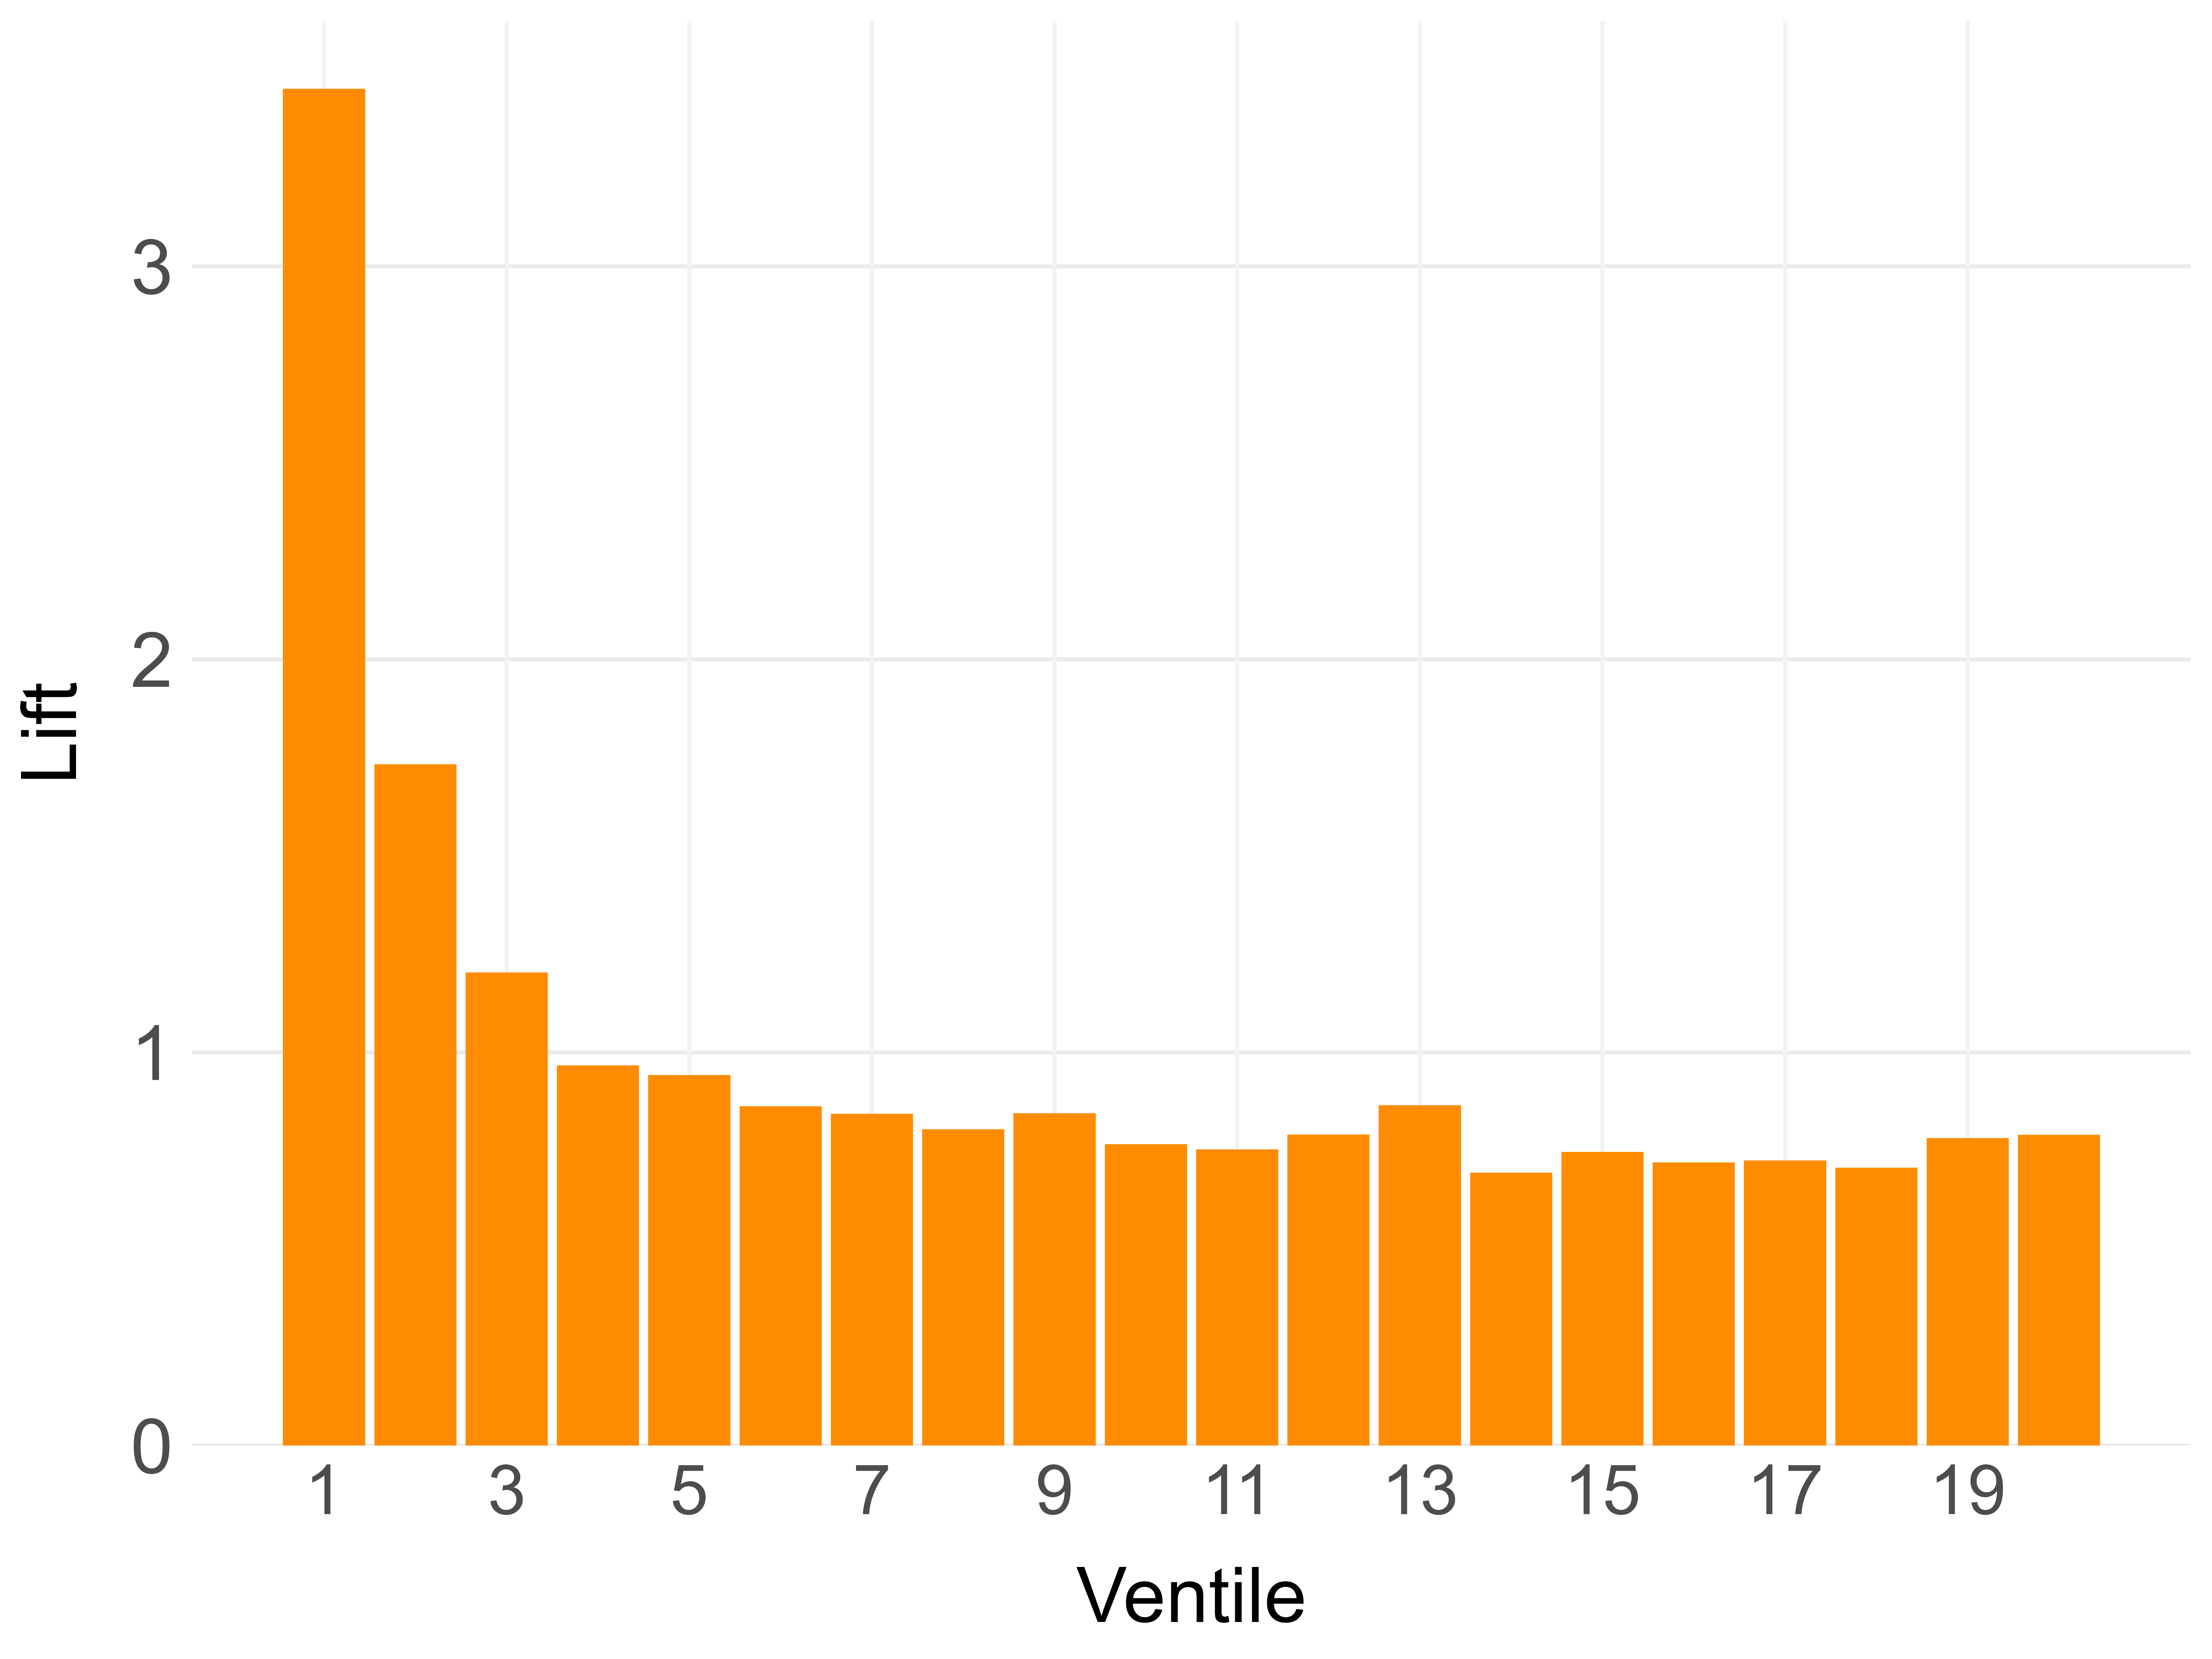
\includegraphics[width=\linewidth]{Figures/winkler_lift_train.png}
  \end{minipage}
  \hfill
  \begin{minipage}{0.43\linewidth}
    \centering
    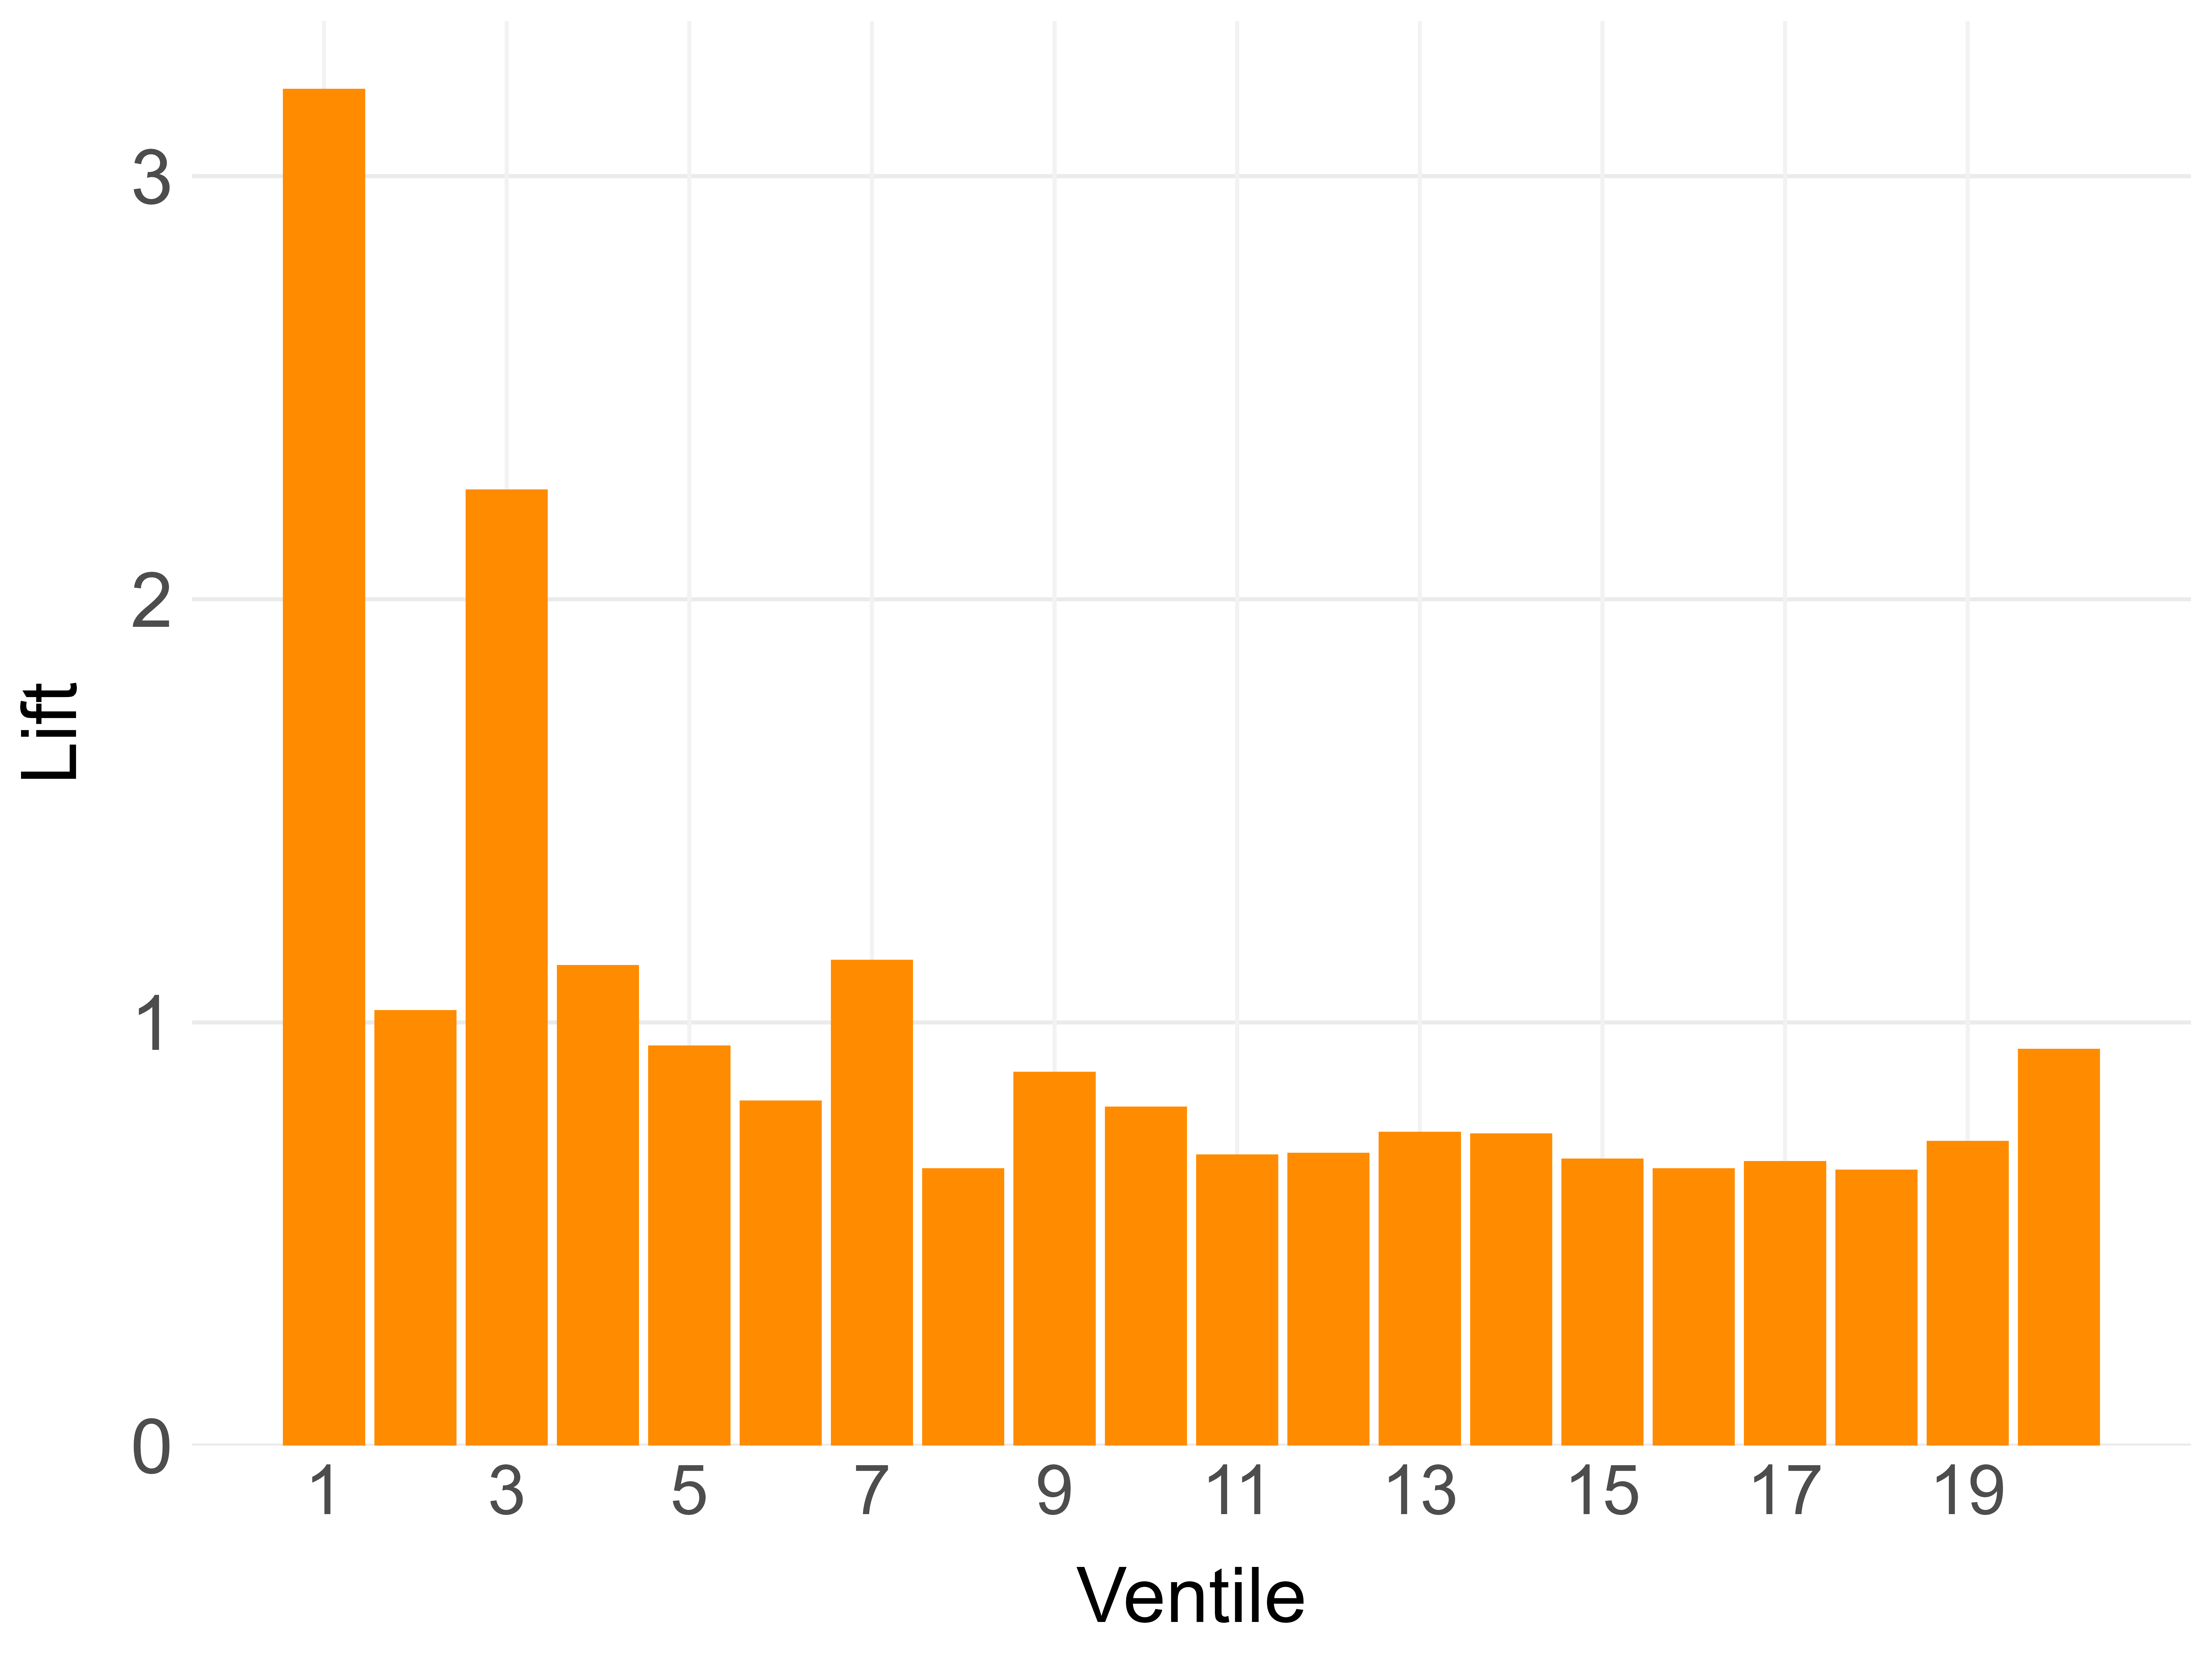
\includegraphics[width=\linewidth]{Figures/winkler_lift_test.png}
  \end{minipage}
  \caption{Lift chart for heart rate training data (left) and test data (right).}
  \label{fig:winkler_lift_test}
\end{figure}

Figure~\ref{fig:winkler_full} displays the heart rate series with flagged periods corresponding to the retained rules. Flagged timestamps align with periods where observed heart rate values frequently fall near or outside the predictive intervals. Rules 1 and 2 reliably flag periods of elevated Winkler scores in both training and test. Rule 3 flagged periods with low values, suggesting it may have overfit to a false pattern in the training data.

\begin{figure}[H]
  \centering
  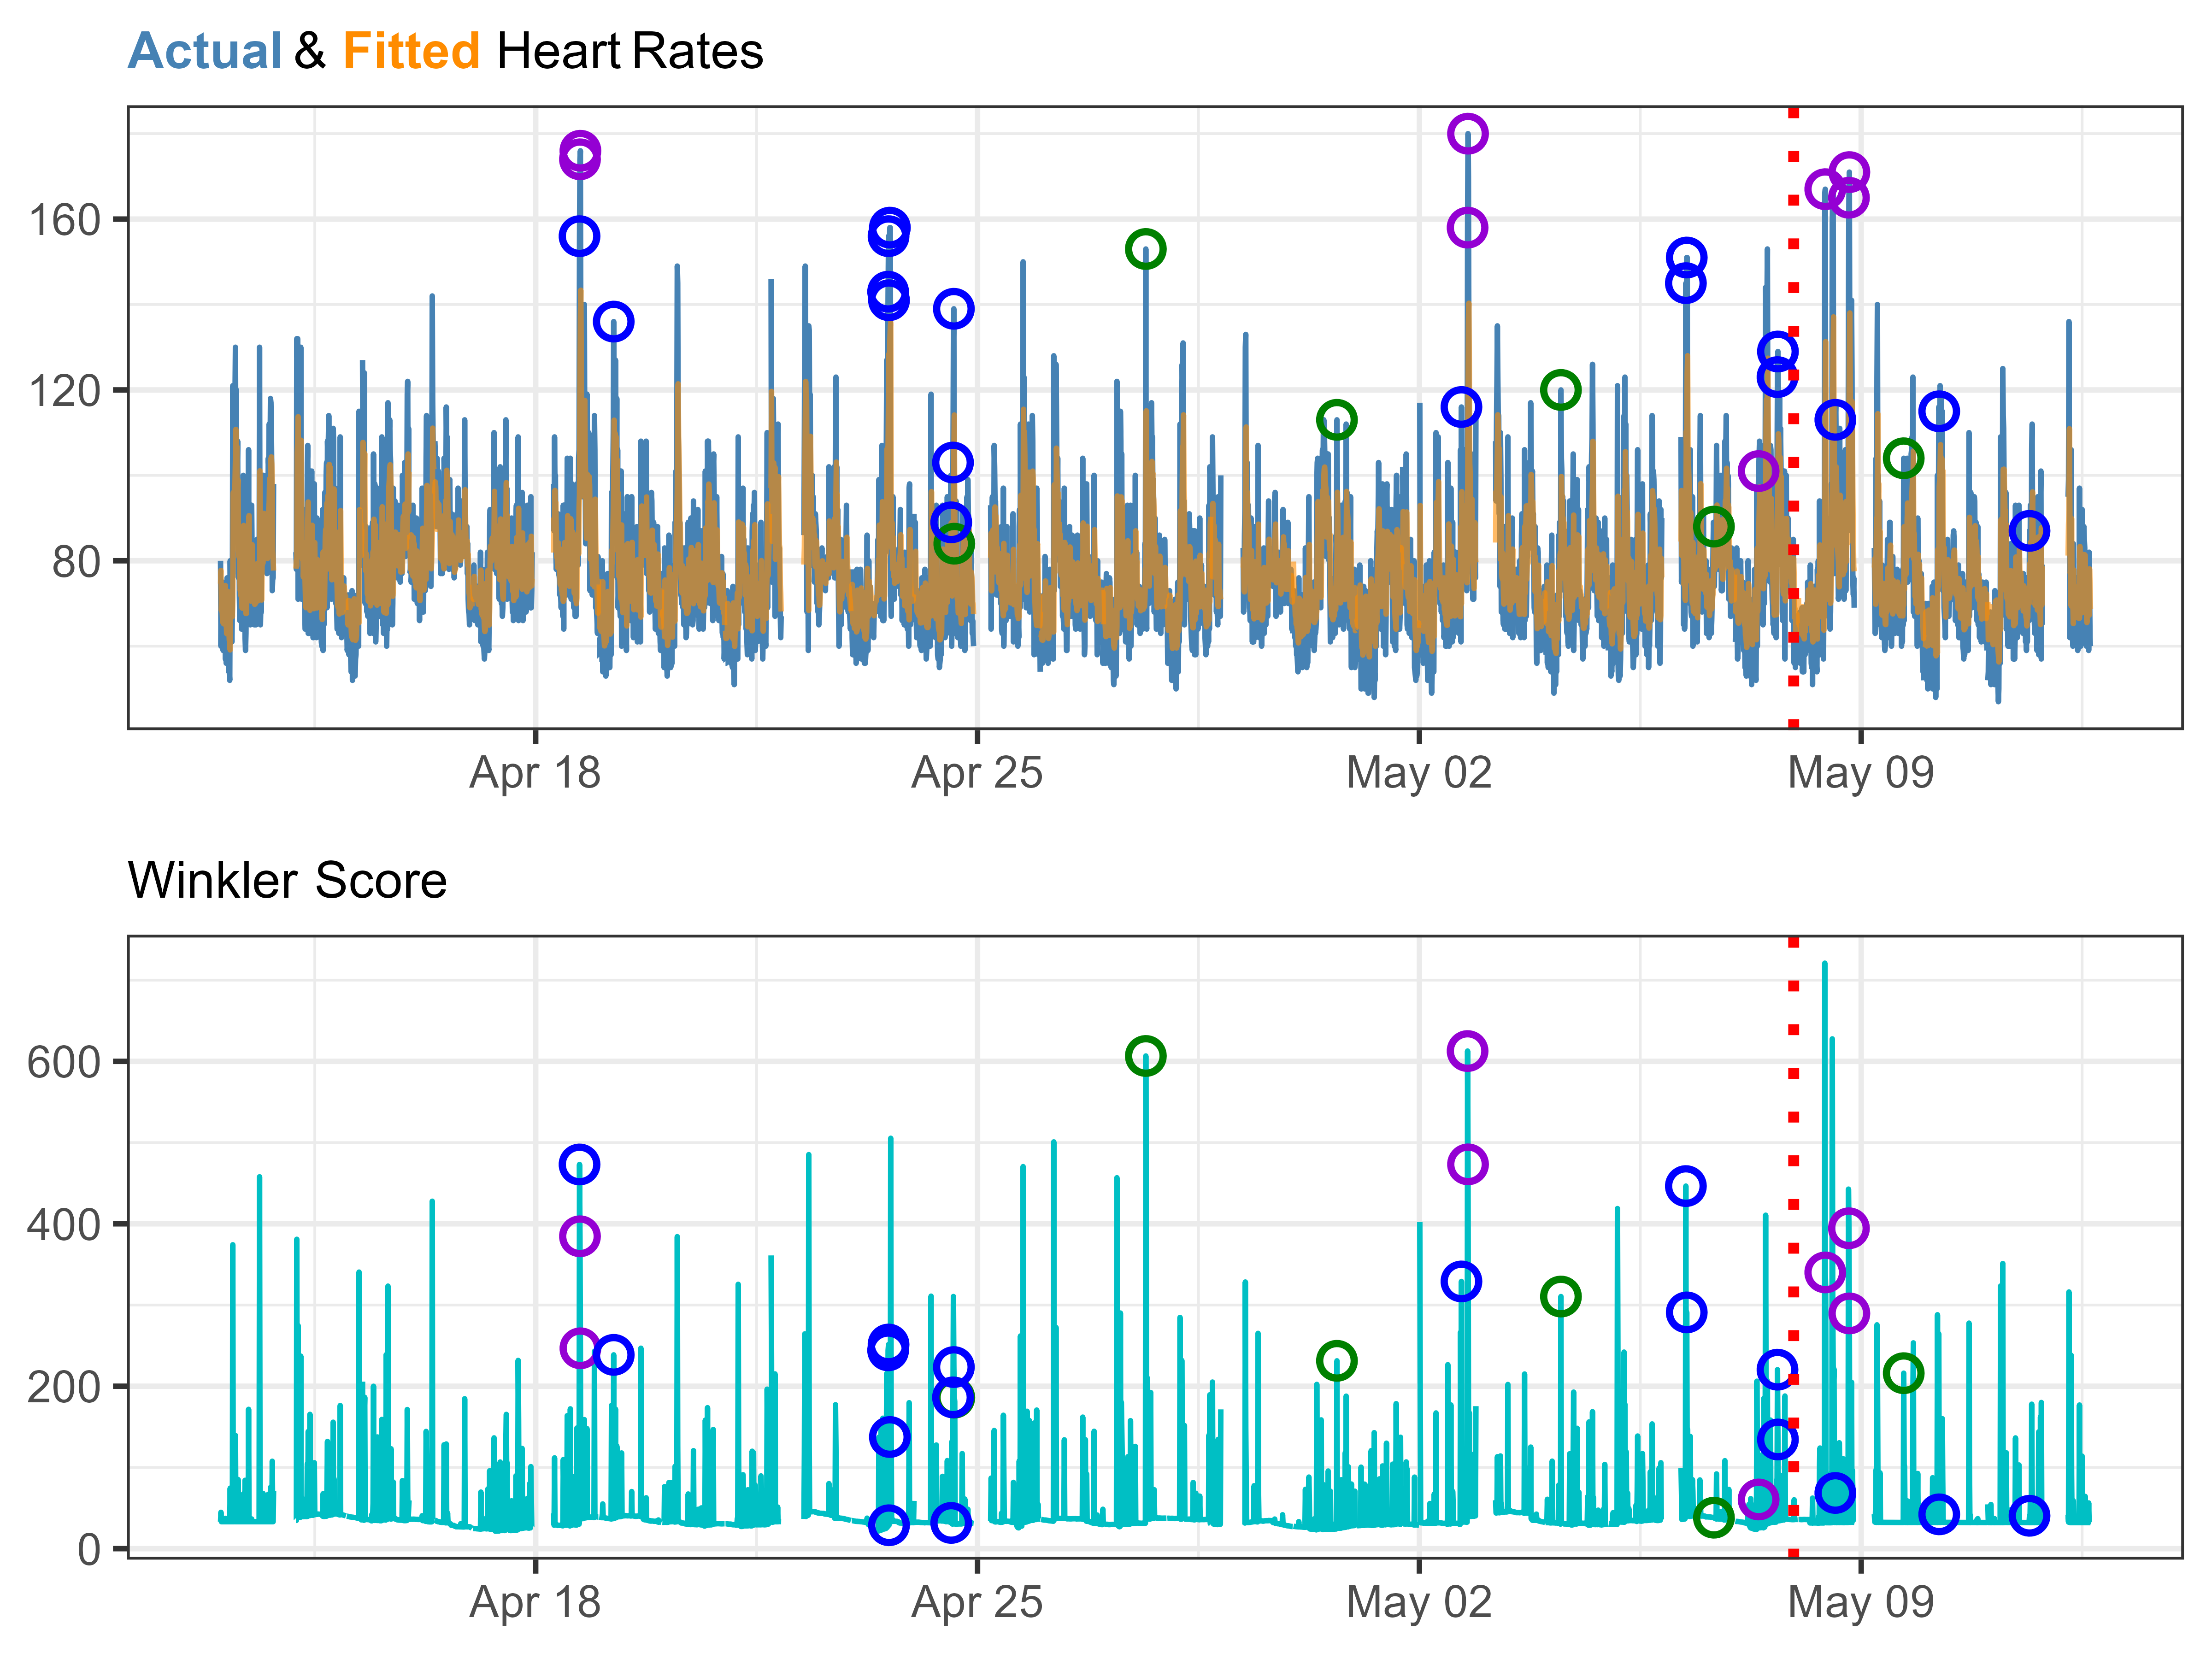
\includegraphics[width=0.9\linewidth]{Figures/winkler_full.png}
  \caption{Heart rate series with flagged periods under Winkler-score TreeAlert.}
  \label{fig:winkler_full}
\end{figure}

\section{Rule Selection for Over- and Under-Forecasting}
\label{append-A}

When domain considerations prioritize predicting both extreme over- and under-forecast failure patterns, TreeAlert can be set to retain both positive and negative mean error rules rather than the most extreme absolute mean errors. This section supplements Section~3.4 (Step~4 -- Rule Extraction and Filtering) and Section~3.5 (Step~5 -- Rule Visualization) by illustrating a variant of the Rule Extraction and Filtering step.

In the electricity demand example, choosing the top-$k$ terminal nodes by absolute mean error resulted in only under-forecast patterns due to their mean magnitudes being most dominant. To reveal over-forecast patterns as well, we partition terminal nodes by the sign of their mean error and then rank separately within each partition. Formally, let $\bar{e}_j$ denote the mean error for terminal node $j$. Define $P=\{j:\bar{e}_j>0\}$ as the set of rules representing \textit{under-forecasting} patterns (positive mean error), and $N=\{j:\bar{e}_j<0\}$ as the set representing \textit{over-forecasting} patterns (negative mean error). We order $P$ in descending $\bar{e}_j$ and $N$ in ascending $\bar{e}_j$, and retain the top $k_1$ nodes from $P$ and the top $k_2$ nodes from $N$ to form the final rule set:
\begin{equation}
\mathcal{R} = \{\, r_j \;|\; j \in P_{k_1} \cup N_{k_2} \,\},
\end{equation}
where $r_j$ denotes the decision rule associated with terminal node $j$, and $P_{k_1}$ and $N_{k_2}$ are the index sets of the top $k_1$ under-forecasting and top $k_2$ over-forecasting nodes, respectively. The total number of retained rules is $k = k_1 + k_2$.

This alternative filtering method ensures the top-$k$ list is not monopolized by a single error direction and addresses cases where dips are not flagged because their node means are smaller in magnitude than peaks (or vice versa). However, this adjustment comes at the cost of retaining rules that predict less extreme errors.

To illustrate, we revisit the electricity demand demonstration, selecting the three nodes with the highest positive average errors and the three with the lowest negative average errors ($k_1 = k_2 = 3$, yielding $k = 6$) while holding all other parameters constant. The six resulting rules are displayed in Table~\ref{tab:treealert_rules} and visualized in Figure~\ref{fig:3x3}.

\begin{table}
\caption{Tree rules for terminal nodes with top three positive and negative mean errors}
\label{tab:treealert_rules}
\small
\centering
\begin{tabular}{r p{11cm}}
\hline
\textbf{Avg.~Error} & \textbf{Rule (Interpreted)} \\
\hline
$4621.59$  & The model under-forecasts by an average of 4622 when Day of Week is Sunday--Monday, Hour is 5PM--6PM, and Minute is 0--14. \\
$3757.46$  & The model under-forecasts by an average of 3757 when Day of Week is Tuesday--Saturday, Hour is 5PM--7PM, and Minute is 15--44. \\
$3626.57$  & The model under-forecasts by an average of 3627 when Day of Week is Sunday--Wednesday, Hour is 2AM and 12AM, and Minute is 15--44. \\
$-1398.24$ & The model over-forecasts by an average of 1398 when Day of Week is Sunday, Hour is 2PM, and Minute is 0--14 and 30--59. \\
$-606.43$  & The model over-forecasts by an average of 606 when Day of Week is Sunday, Hour is 3PM, and Minute is 0--14 and 30--59. \\
$-534.00$  & The model over-forecasts by an average of 534 when Day of Week is Sunday, Hour is 1PM and 4PM, and Minute is 0--14. \\
\hline
\end{tabular}
\end{table}

\clearpage
\noindent
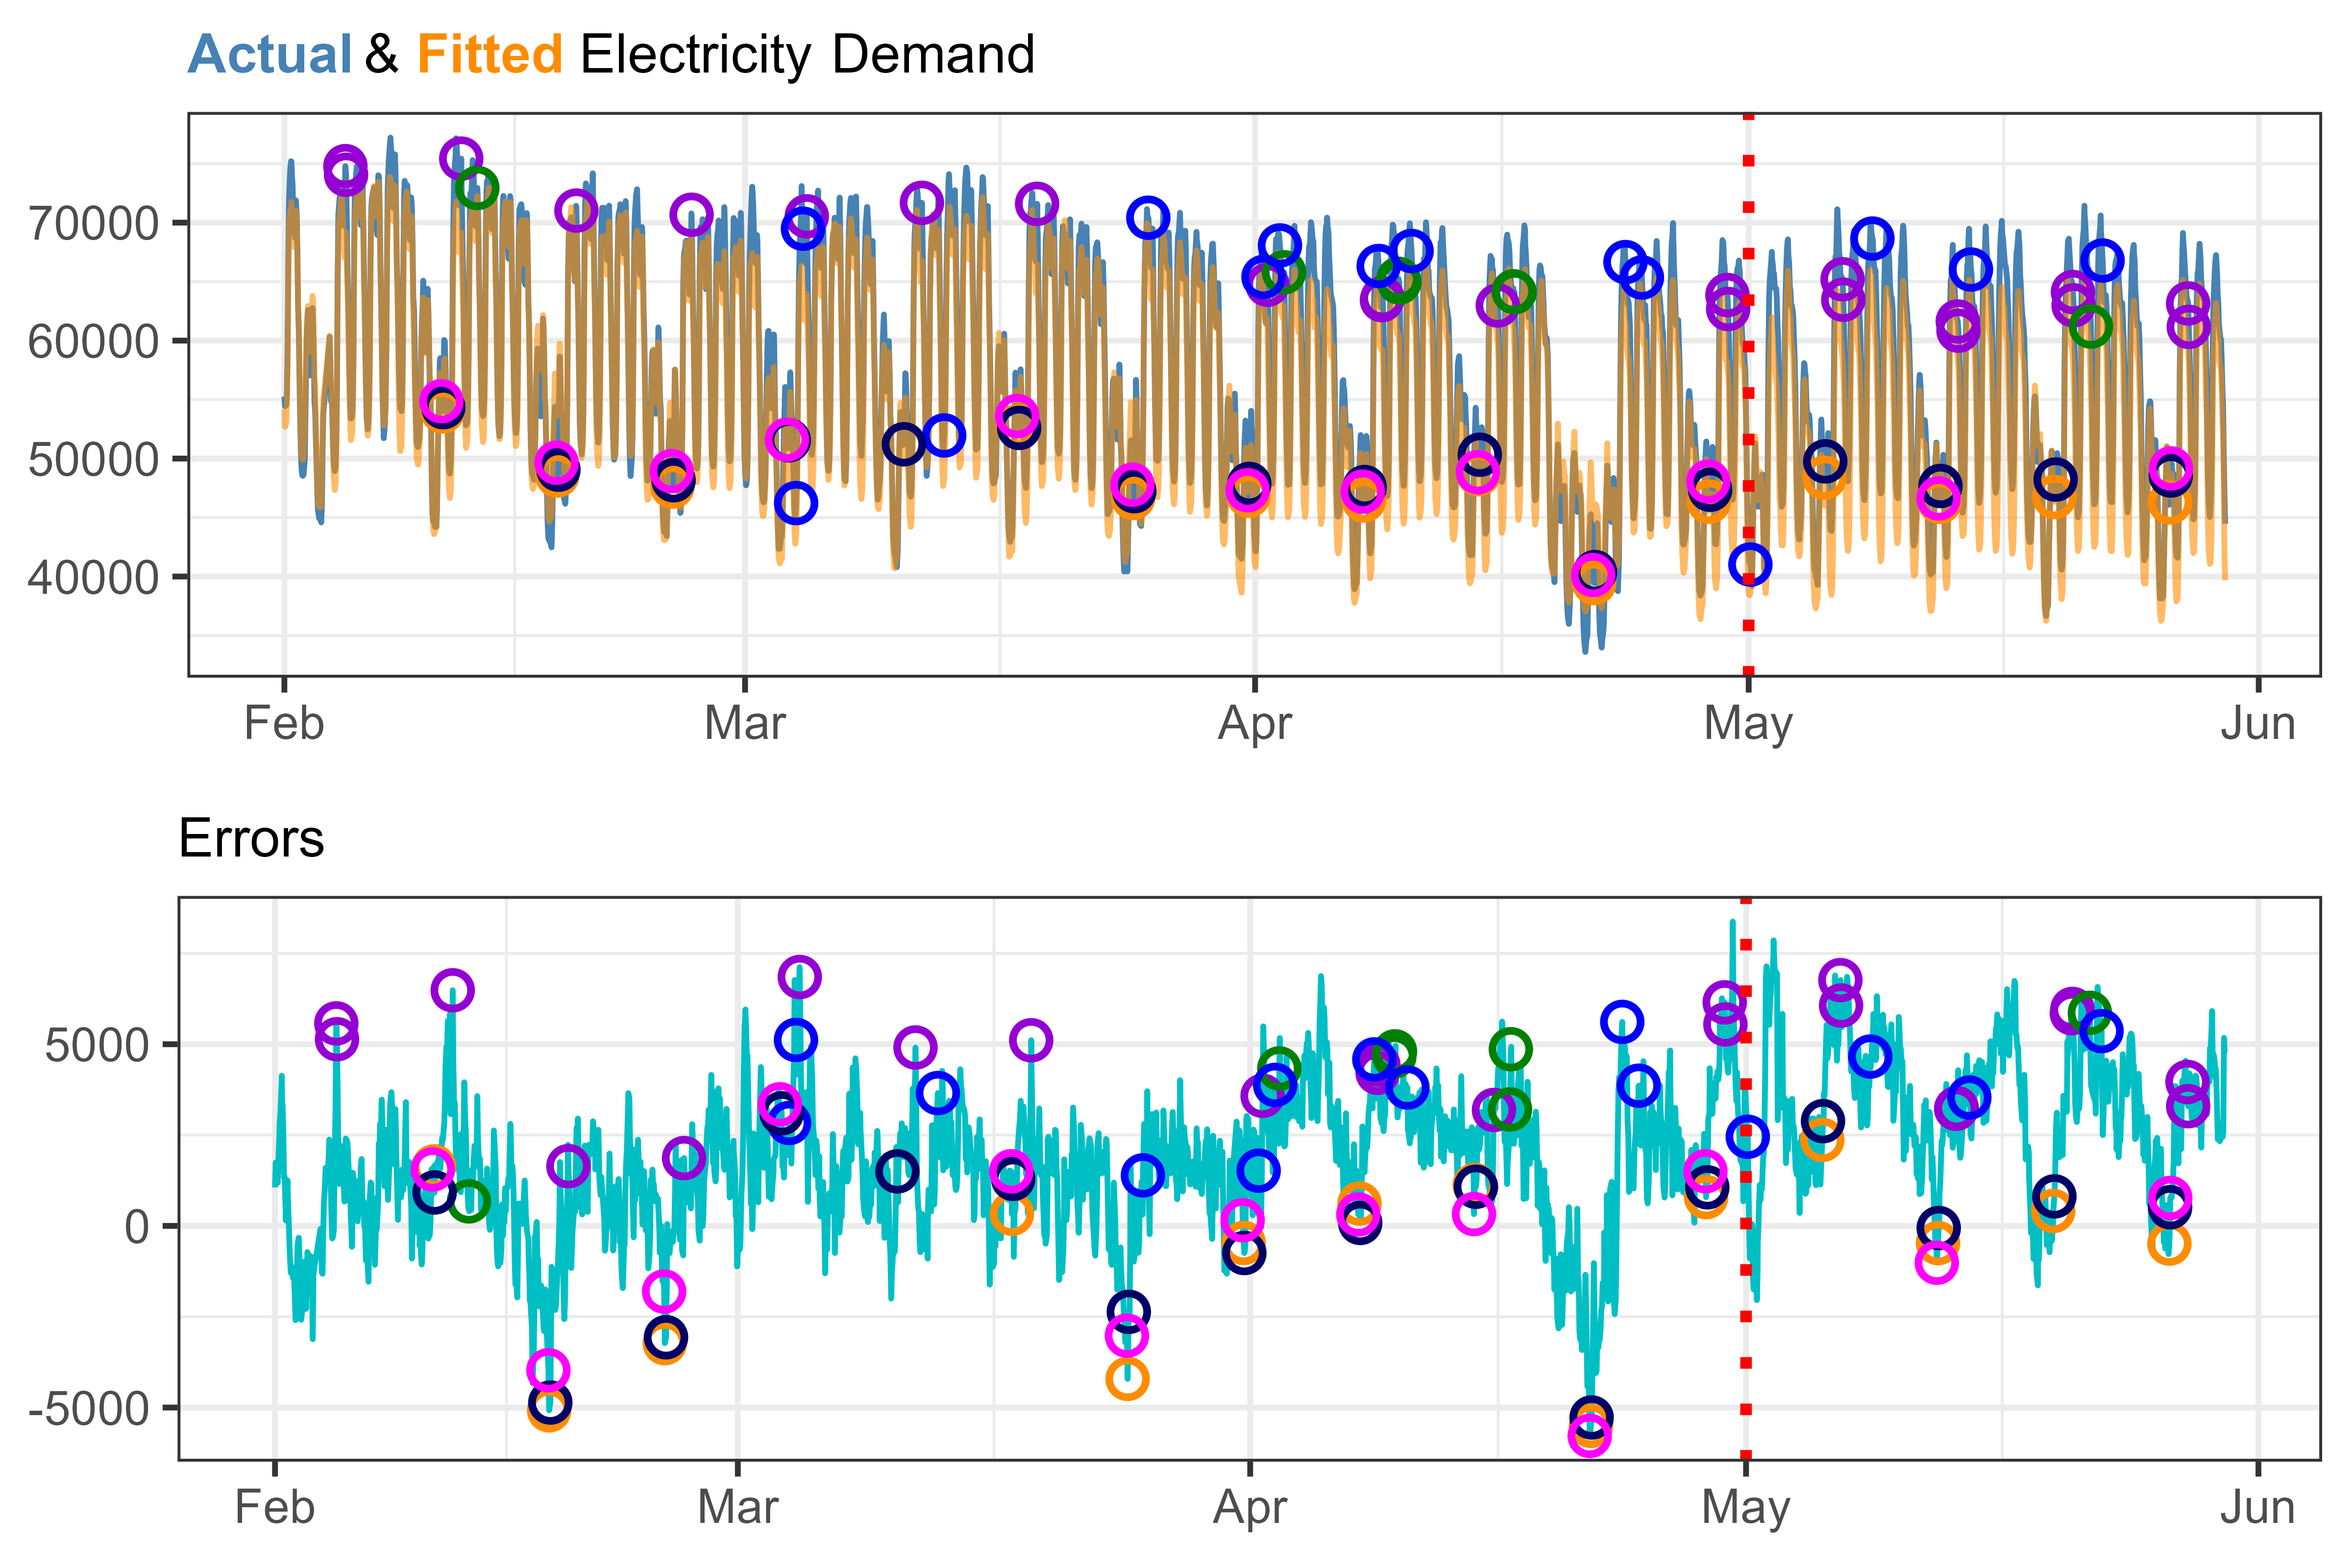
\includegraphics[width=\linewidth]{Figures/Elec_3x3_both.png}
\captionof{figure}{Example of TreeAlert retaining both positive and negative mean error rules.}
\label{fig:3x3}

\end{document}
